\documentclass[../main.tex]{subfiles}
\begin{document}
\newpage
\section{Приближенное решение задачи синтеза управления на малом интервале времени}
\subsection{Асимптотика множеств достижимости нелинейных систем с интегральными ограничениями, в том числе по части координат} 
Данный раздел содержит материалы, опубликованные в статье И. О. Осипов, “О выпуклости множеств достижимости по части координат нелинейных управляемых систем на малых промежутках времени”, Вестн. Удмуртск. ун-та. Матем. Мех. Компьют. науки, 31:2 (2021),  210–225. В разделе исследована выпуклость множеств достижимости по части координат нелинейных систем с интегральными ограничениями на управление на малых промежутках времени.
Доказаны достаточные условия выпуклости, имеющие вид ограничений на асимптотику собственных чисел грамиана управляемости линеаризованной системы по части координат.
В качестве примеров, в статье описаны две нелинейные системы третьего порядка, в одной из которых линеаризованная вдоль траектории, порожденной нулевым управлением, система неуправляема, а в другом управляема.
Исследованы достаточные условия выпуклости проекций множеств достижимости. 
Проведено численное моделирование, продемонстрировавшее невыпуклость некоторых проекций даже для малых длин временного промежутка.
\subsubsection{Расстояние Банаха-Мазура и асимптотическая эквивалентность множеств}
Напомним, что расстоянием Банаха-Мазура между выпуклыми компактными множествами $ X,Y \subset \mathbb R^n $ называют величину $ \rho (X, Y)  $, определенную равенством 
\begin{gather*}
	\rho (X, Y): = \log (r(X,Y) \cdot r(Y, X)),
\end{gather*}
где $r(X, Y) = \inf \{t \geq 1: tX \supset Y \}$.\\
Пусть $ X = X(\varepsilon) $,  $ Y = Y(\varepsilon) $ -- выпуклые компактные множества, такие, что $ 0 \in \rm{int}\,X(\varepsilon) $, $ 0 \in \rm{int}\,Y(\varepsilon) $ при $0 \leqslant \varepsilon \leqslant \overline{\varepsilon} $.  Тогда, следуя \footnote{Goncharova E., Ovseevich A. Small-time reachable sets of linear systems with integral control constraints: birth of the shape of a reachable set// Journal of Optimization Theory and Applications. 2016. 168 (2). P. 615--624.
	doi: 10.1007/s10957-015-0754-4}, назовем множества $  X(\varepsilon)  $ и $  Y(\varepsilon) $ {\textit асимптотически эквивалентными}, если $  \rho (X(\varepsilon), Y(\varepsilon)) \rightarrow 0 $ при $\varepsilon \rightarrow 0 $.

Приведем далее достаточное условие асимптотической эквивалентности, выраженное через хаусдорфово расстояние $ h $ между ними.
\begin{theorem}\label{suff}\footnote{Gusev M.I. The limits of applicability of the linearization method in calculating small-time reachable sets // Ural Mathematical Journal. 2020. Vol. 6, No. 1. P. 71-83 https://doi.org/10.15826/umj.2020.1.006}
	 Выполнения следующих условий достаточно для того, чтобы множества $ X(\varepsilon) $ и $ Y(\varepsilon) $ были асимптотически эквивалентны:
	\begin{gather*}
		\lim\limits_{\varepsilon \rightarrow 0}h(X(\varepsilon),Y(\varepsilon)) = 0, \qquad	\lim\limits_{\varepsilon \rightarrow 0}\frac{h(X(\varepsilon),Y(\varepsilon))}{\delta_{min}(Y(\varepsilon))} = 0,
	\end{gather*}
	где $ \delta_{min}(Y(\varepsilon)) = \inf\limits_{\left\|y \right\| =1 } \delta(y|Y(\varepsilon))$, а $ \delta(y|Y(\varepsilon)) $ -- опорная функция множества $ Y(\varepsilon) $.
\end{theorem}
\subsubsection{Достаточное условие асимптотической эквивалентности множеств достижимости нелинейной и линеаризованной систем}
	Рассмотрим нелинейную систему, аффинную по управлению
\begin{gather}\label{nonlinearY}
	\begin{gathered}
		\dot{x}(t)=f_1(t,x(t))+f_2(t,x(t))u(t), \qquad t_0 \leq t \leq t_0 + \bar{\varepsilon}, \qquad x(t_0) = x_0, \\
		y(t) = C x(t).
	\end{gathered}
\end{gather}
Здесь $ x \in \mathbb{R}^n $ -- вектор состояния, $ u \in \mathbb{R}^r $ -- управление,  $ y\in\mathbb{R}^m (m \leqslant n) $ -- выход системы,
$ C\in \mathbb{R}^{m \times n} $  -- матрица полного ранга, $m\leq n$, $ \bar{\varepsilon} $ --- некоторое фиксированное положительное число.
	Как и в предыдущих разделах функции $ f_1: \mathbb{R}^{n+1} \rightarrow \mathbb{R}^{n} $, $ f_2: \mathbb{R}^{n+1} \rightarrow \mathbb{R}^{n \times r} $ предполагаются непрерывными и непрерывно-дифференцируемыми по $ x $.
По-прежнему предполагается, что функции $ f_1 $, $ f_2 $ удовлетворяют условиям
\begin{gather*}
	\begin{gathered}
		\left\| f_1(t,x) \right\| \leqslant	l_1(t)(1 + \left\| x \right\| ), \\
		\left\| f_2(t,x) \right\| \leqslant	l_2(t),  \qquad t_0 \leqslant t \leqslant t_0 + \bar{\varepsilon}, \qquad   x \in \mathbb{R}^n,
	\end{gathered}
\end{gather*}
где $ l_1(\cdot) \in \mathbb{L}_1[t_0,t_0+\bar{\varepsilon}] $, $ l_2(\cdot) \in \mathbb{L}_2[t_0,t_0+\bar{\varepsilon}] $. Предположение \ref{Pred} также считается выполненным.

 Управление $u(t)$ будем выбирать из
пространства $\mathbb{L}_2[t_0,t_0+\bar{\varepsilon}]$ вектор-функций и ограничим его шаром радиуса $ \mu > 0 $
\begin{gather}\label{constrY}
	\lVert u(\cdot)\rVert^2_{\mathbb{L}_2} = \left(u(\cdot),u(\cdot) \right) \leqslant \mu^2.
\end{gather}

В условиях описанных предположений, каждому $ u(\cdot) \in \mathbb{L}_2 $ соответствует единственное абсолютно непрерывное решение $ x(t)=x(t,u(\cdot)) $ системы \eqref{nonlinearY}, определённое на интервале $ [t_0,t_0+\bar{\varepsilon}] $.

Все траектории $ x(t) $ системы \eqref{nonlinearY}, отвечающие удовлетворяющим \eqref{constrY} управлениям,  лежат внутри некоторого компактного множества $ D \subset \mathbb{R}^n $. Пусть $ 0 <  \varepsilon \leqslant \bar{\varepsilon} $. 

Множеством достижимости системы \eqref{nonlinearY} по состоянию, как и прежде, будем называть множество \begin{gather*}
	G(\varepsilon)=\{x\in \mathbb{R}^n:\exists u(\cdot)\in B_{\mathbb{L}_2}(0,\mu),\; x=x(t_0+\varepsilon,x^0,u(\cdot))\}.
\end{gather*}


\begin{definition}
	{\textit Множеством достижимости $G_y(\varepsilon)$ системы \eqref{nonlinear} по выходу} $ y = C x $ будем называть множество всех выходов $ y(t_0+\varepsilon) $,
	соответствующих концам траекторий $ x(t_0+\varepsilon) $, порождённых управлениями $ u(t) \in B_{\mathbb{L}_2}(0,\mu)$
	\begin{gather*}
		G_y(\varepsilon)=\{y\in \mathbb{R}^m:\exists u(\cdot)\in B_{\mathbb{L}_2}(0,\mu),\; y=Cx(t_0+\varepsilon,x^0,u(\cdot))\}.
	\end{gather*}
\end{definition}

В определениях множеств, приведённых выше, можно считать, что $ \mathbb{L}_2 =\mathbb{L}_2[t_0,t_0+\varepsilon] $, либо  $ \mathbb{L}_2=\mathbb{L}_2[t_0,t_0+\bar{\varepsilon}] $. Нетрудно понять, что для любого из этих пространств мы получаем одно и то же множество достижимости. Будем далее считать, что $ \mathbb{L}_2 =\mathbb{L}_2[t_0,t_0+\varepsilon] $.
	
Заметим, что  $ G_y(\varepsilon) = C G(\varepsilon) $.	
	
Если матрица $ C \in \mathbb{R}^{m \times n} $ такова, что в каждой её строке только один элемент равен 1, а остальные равны 0, а в каждом столбце содержится не более одного ненулевого элемента, то $ y=Cx $ состоит из $ m$ координат вектора $ x $, а  множество достижимости $G_y(\varepsilon)$ представляет собой проекцию множества $ G(\varepsilon) $ на $m$--мерную координатную плоскость.


\begin{definition}
	Симметричная матрица, определённая равенством
	\begin{gather*}
		W_y(\varepsilon) = C\int_{t_0}^{t_0+\varepsilon}X(t_0+\varepsilon,t)B(t)B^{\top}(t)X^{\top}(t_0+\varepsilon,t) \, dtC^\top=CW(\varepsilon)C^\top,
	\end{gather*}
	называется грамианом управляемости системы \eqref{linear} на интервале времени $  t_0 \leq t \leq t_0 + \varepsilon $ по выходу $y$.
\end{definition}
	
	Система \eqref{linear} вполне управляема на  $ [t_0, t_0 + \varepsilon] $ по выходу $y=Cx$ тогда и только тогда,
	когда  грамиан управляемости по выходу $ \widetilde{W}_y(\varepsilon) = C \widetilde{W}(\varepsilon) C^{\top}  $ -- положительно определенная матрица, то есть его минимальное собственное число $ \nu^y(\varepsilon) $ положительно.
	
	Основной результат этого раздела отражен в следующей теореме.
	\begin{theorem}\label{th2}
		При достаточно малых $ \varepsilon $ множество достижимости $ G_y(\varepsilon) $ системы \eqref{nonlinear} по выходу $ y = C x $ выпукло и асимптотически эквивалентно множеству $W_y^{1/2}(\varepsilon)B_{\mathbb{R}^n}(0,\mu) + Cx(t_0+\varepsilon,0)$, если найдутся такие $ K>0 $, $ \alpha > 0 $, $ 0< \varepsilon_0<\overline{\varepsilon}  $, что для всех $ \varepsilon \leqslant \varepsilon_0 $
		\begin{gather}\label{cond1}
			\nu^y(\varepsilon) \geqslant \left\{ {\begin{array}{*{20}{l}}
					{K\varepsilon ^{3 - \alpha}, \mbox{\ если \ } f_2(t,x) \mbox{\ не зависит от \ } x}, \\
					{K\varepsilon ^{1 - \alpha}}, \mbox{\ в противном случае}.
			\end{array}} \right.
		\end{gather}
	\end{theorem}
	
	Здесь $W_y^{1/2}(\varepsilon)$ --- арифметический квадратных корень из матрицы $W_y(\varepsilon)$, $ B_{\mathbb{R}^n}(0,\mu) $ --- евклидов шар радиуса $ \mu $ в $ \mathbb{R}^n $
	
	\doc. 
	При фиксированном $ \varepsilon $ введем отображение $ F_{\varepsilon}: \mathbb{L}_2[0,1]  \rightarrow \mathbb{R}^n$, зависящее от параметра $ \varepsilon $ равенством $F_{\varepsilon}(\upsilon(\cdot)) = z(1,\upsilon(\cdot)) $, где  $ z(\tau,\upsilon(\cdot)) $ -- траектория системы \eqref{epsnonlinear}, соответствующая управлению $ \upsilon(\cdot) $. Тогда композиция отображений $ F_{\varepsilon}$ и $ C $, $ H_{\varepsilon}: \mathbb{L}_2[0,1]  \rightarrow \mathbb{R}^k $, есть $ H_{\varepsilon}(\upsilon(\cdot)) = CF_{\varepsilon}(\upsilon(\cdot)) = Cz(1,\upsilon(\cdot)) $. В силу \eqref{epscond}, мы имеем $ H_{\varepsilon}(B_{\mathbb{L}_2[0,1]}(0,\varrho(\varepsilon))) = \widetilde{G}_y(\varepsilon) = G_y(\varepsilon)  $, где $ \varrho(\varepsilon) = \mu \sqrt{\varepsilon} $.
	
	Отображение $ H_{\varepsilon} $ непрерывно дифференцируемо по Фреше для $ \forall \upsilon(\cdot) \in  B_{\mathbb{L}_2[0,1]}(0,\varrho(\varepsilon)) $, как композиция непрерывно дифференцируемых отображений и его производная Фреше $ H_{\varepsilon}': \mathbb{L}_2[0,1]  \rightarrow  \mathbb{R}^k $ определена равенством:
	\begin{gather*}
		H_{\varepsilon}'( \upsilon(\cdot))\delta \upsilon = C \delta z(1) = C F_{\varepsilon}'(\upsilon(\cdot))\delta  \upsilon,
	\end{gather*}
	где $ \delta z(1) $ --- решение линеаризованной системы \eqref{epslinear} c нулевыми начальными условиями и управлением $  \delta  \upsilon(\tau) $, $ F_{\varepsilon}'( \upsilon(\cdot)) $ --- производная Фреше отображения $ F _{\varepsilon}$.
	Для $ F_{\varepsilon}' $ имеет место равенство (см., например \footnote{Gusev M.I. Estimates of the minimal eigenvalue of the controllability Gramian for a system containing a small parameter//  Mathematical Optimization Theory and Operations Research. Lecture Notes in Computer Science. 2019. vol. 11548. P. 461--473.  https://doi.org/10.1007/978-3-030-22629-9\_32}).
	\begin{equation}\label{derivF}
		F_{\varepsilon}'( \upsilon(\cdot)) = X_{\varepsilon}(1,\tau, \upsilon(\cdot))B_{\varepsilon} (\tau, \upsilon(\cdot)), \quad \tau\in[0,1],
	\end{equation}
	где $ X_{\varepsilon}(1,\tau,\upsilon(\cdot)) $ --- фундаментальная матрицы системы \eqref{epslinear}, матрицы которой $ A_{\varepsilon}(\tau) $, $ B_{\varepsilon}(\tau)  $ зависят от $ \upsilon(\cdot) $.
	Из \eqref{derivF} следует, что $ H_{\varepsilon}'(u(\cdot)) $ есть ни что иное, как
	\begin{equation*}
		H_{\varepsilon}'(\upsilon(\cdot)) = C X_{\varepsilon}(1,\tau, \upsilon(\cdot))B_{\varepsilon} (\tau, \upsilon(\cdot)), \quad \tau\in[0,1],
	\end{equation*}
	Можно доказать, что $ F_{\varepsilon}'(\upsilon(\cdot)) $ --- липшицева
	\begin{equation}\label{lipdF}
		\left\| F_{\varepsilon}'(\upsilon_1(\cdot)) - F_{\varepsilon}'(\upsilon_2(\cdot)) \right\| \leqslant L(\varepsilon) \left\| \upsilon_1(\cdot) - \upsilon_2(\cdot)\right\|
	\end{equation}
	при $ \upsilon \in B_{\mathbb{L}_2[0,1]}(0,\rho(\varepsilon))  $, но тогда и $ H_{\varepsilon}'(\upsilon(\cdot)) $ --- липшицева. Доказательство проводится по схеме работы\footnote{Gusev M.I. The limits of applicability of the linearization method in calculating small-time reachable sets // Ural Mathematical Journal. 2020. Vol. 6, No. 1. P. 71-83 https://doi.org/10.15826/umj.2020.1.006}.  При этом $ L(\varepsilon) = L_0 + L_1 \varepsilon $, где $ L_0 = 0$, если $ f_2(t,x)  $ не зависит от $ x $.
	Тогда можно оценить максимальный радиус $ \rho(\varepsilon) $ гильбертова шара $ B_{\mathbb{L}_2[0,1]}(0,\rho(\varepsilon)) $, образ которого $ F_{\varepsilon}(B_{\mathbb{L}_2[0,1]}(0,\rho(\varepsilon))) $ будет выпуклым (см. \footnote{Polyak B.T. Сonvexity of the reachable set of nonlinear
		systems under l2 bounded controls // Dynamics of Continuous, Discrete and Impulsive Systems
		Series A: Mathematical Analysis. 2004. Vol. 11.  P. 255--267.}):
	\begin{equation}\label{Polest}
		\rho(\varepsilon) \leqslant \frac{\sqrt{\nu(\varepsilon)}}{2L(\varepsilon)}.
	\end{equation}
	Теперь проведем аналогичные рассуждения для $ H_{\varepsilon} $. Аналог неравенства \eqref{lipdF}  имеет вид
	\begin{equation*}
		\left\| H_{\varepsilon}'(\upsilon_1(\cdot)) - H'_{\varepsilon}(\upsilon_2(\cdot)) \right\| \leqslant L(\varepsilon) \left\| \upsilon_1(\cdot) - \upsilon_2(\cdot)\right\|,
	\end{equation*}
	где для константы Липшица $ L(\varepsilon) = L_0 + L_1 \varepsilon$ отображения $ H_{\varepsilon} $ сохраним то же обозначение, что и в \eqref{lipdF}.
	А неравенство \eqref{Polest} перепишем так, чтобы найти условие, при котором множество достижимости системы \eqref{epsnonlinear} по выходу $ \widetilde{G}_y(1) = H_{\varepsilon} (B_{\mathbb{L}_2[0,1]}(0,\varrho(\varepsilon)))$ будет выпуклым:
	\begin{equation}\label{est2}
		4\varrho^2(\varepsilon)L^2(\varepsilon) = 4\mu^2\varepsilon L^2(\varepsilon) \leqslant \nu^y(\varepsilon),
	\end{equation}
	где $ \varrho(\varepsilon)  = \mu\sqrt{\varepsilon} $.
	
	В случае, если функция $ f_2(t,x) $ не зависит от $ x $, то $ L(\varepsilon) = L_1 \varepsilon  $, а \eqref{est2} принимает вид $ \nu^y(\varepsilon) \geqslant 4\mu^2L_1^2 \varepsilon^3 $.  Это неравенство будет выполнено, если $ K\varepsilon^{3 - \alpha} \geqslant 4\mu^2L_1^2 \varepsilon^3 $, что равносильно соотношению $ \varepsilon \geqslant \varepsilon_1 := \left(\frac{K}{4\mu^2L_1^2}\right)^{1/\alpha} $.  Таким образом, множество достижимости $ G_y(\varepsilon)$ выпукло при $ 0 \leqslant \varepsilon \leqslant \min\{\varepsilon_0,\varepsilon_1\}  $.  
	
	В другом случае, если $ f_2(t,x) $ зависит от $ x $, $ L(\varepsilon) =L_0+L_1\varepsilon $, а \eqref{est2} принимает вид $ \nu^y(\varepsilon) \geqslant 4\mu^2 \varepsilon (L_0 + L_1 \varepsilon)^2 $.  Учитывая, что $ \nu^y(\varepsilon)  \geqslant K \varepsilon^{1-\alpha} $, достаточно доказать, что $ K \varepsilon^{1-\alpha}  \geqslant 4\mu^2 \varepsilon (L_0 + L_1 \varepsilon_0)^2 $. Последнее неравенство выполняется при $ \varepsilon \leqslant \varepsilon_2 := \left(\frac{K}{4\mu^2(L_0 + L_1\varepsilon_0)^2} \right)^{1/\alpha} $. Следовательно, $ G_y(\varepsilon) $ выпукло, если $ 0 \leqslant \varepsilon \leqslant \min\{\varepsilon_0, \varepsilon_2\} $.
	
	Множество $ W_y^{1/2}(\varepsilon)B_{\mathbb{R}^n}(0,\mu) + Cx(t_0+\varepsilon,0)  = H'_{\varepsilon}(0)B_{\mathbb{L}_2[0,1]}(0,\varrho(\varepsilon))+ H_{\varepsilon}(0)$ есть не что иное, как множество достижимости по выходу линеаризованной системы \eqref{epslinear}.
	
	Доказательство асимптотической эквивалентности проекций множеств достижимости нелинейной и линеаризованной систем проводится по той же схеме, что и доказательство следствий теоремы 2 в \footnote{Gusev M.I. The limits of applicability of the linearization method in calculating small-time reachable sets // Ural Mathematical Journal. 2020. Vol. 6, No. 1. P. 71-83 https://doi.org/10.15826/umj.2020.1.006}. Оценим сверху хаусдорфово расстояние между образами гильбертова шара $ H_{\varepsilon}\left( B_{\mathbb{L}_2[0,1]}(0,\varrho(\varepsilon))\right)  $ и $ H'_{\varepsilon}(0)B_{\mathbb{L}_2[0,1]}(0,\varrho(\varepsilon))+ H_{\varepsilon}(0) $:
	\begin{gather*}
		h\left( G_y(\varepsilon), H'_{\varepsilon}(0)B_{\mathbb{L}_2[0,1]}(0,\varrho(\varepsilon))+ H_{\varepsilon}(0)\right)  \leqslant L(\varepsilon) \varrho^2(\varepsilon).
	\end{gather*}
	А так как $ \lim\limits_{\varepsilon \rightarrow 0}  L(\varepsilon) \varrho^2(\varepsilon) = 0 $, то и $ \lim\limits_{\varepsilon \rightarrow 0} h\left( G_y(\varepsilon), H'_{\varepsilon}(0)B_{\mathbb{L}_2[0,1]}(0,\varrho(\varepsilon))+ H_{\varepsilon}(0)\right)  = 0 $.
	
	
	Множество достижимости линеаризованной системы -- конечномерный эллипсоид и его наименьшая полуось $ \delta_{min}\left(H'_{\varepsilon}(0)B_{\mathbb{L}_2[0,1]}(0,\varrho(\varepsilon)) \right)=\varrho(\varepsilon)\sqrt{\nu^y(\varepsilon)} $. 
	Следовательно,
	\begin{gather*}
		\frac{h\left(G_y(\varepsilon), H'_{\varepsilon}(0)B_{\mathbb{L}_2[0,1]}(0,\varrho(\varepsilon))+ H_{\varepsilon}(0)\right) }{\delta_{min}\left( H'_{\varepsilon}(0)B_{\mathbb{L}_2[0,1]}(0,\varrho(\varepsilon))\right) } \leqslant \frac{L(\varepsilon) \varrho(\varepsilon)}{\sqrt{\nu^y(\varepsilon)}}.
	\end{gather*}
	
	При выполнении условий \eqref{cond1} в первом случае ($ f_2(t,x) $ не зависисит от $ x $) имеем
	\begin{gather*}
		\frac{L(\varepsilon) \varrho(\varepsilon)}{\sqrt{\nu^y(\varepsilon)}} 
		\leqslant
		\frac{L_1\varepsilon\mu\sqrt{\varepsilon}}{K^{\frac{1}{2}}\varepsilon^{\frac{3}{2}-\frac{\alpha}{2}}} 
		=
		L_1\mu K^{-\frac{1}{2}}\varepsilon^{\frac{\alpha}{2}} \rightarrow 0 \mbox{\ при\ } \varepsilon \rightarrow 0.
	\end{gather*}
	
	Во втором случае,
	\begin{equation*}
		\frac{L(\varepsilon) \varrho(\varepsilon)}{\sqrt{\nu^y(\varepsilon)}} 
		\leqslant
		\frac{(L_0+L_1\varepsilon)\mu\sqrt{\varepsilon}}{{K^{\frac{1}{2}}}\varepsilon^{\frac{1}{2}-\frac{\alpha}{2}}}
		=
		(L_0+L_1\varepsilon)\mu K^{-\frac{1}{2}}\varepsilon^{\alpha/2} \rightarrow 0 \mbox{\ при\ } \varepsilon \rightarrow 0.
	\end{equation*}
	
	Таким образом условия теоремы \ref{suff} выполнены, а значит множества $ G_y(\varepsilon) $ и \\ $ H'_{\varepsilon}(0)B_{\mathbb{L}_2[0,1]}(0,\varrho(\varepsilon))+ H_{\varepsilon}(0) $ асимптотически эквиваленты.
	\hfill $\square$
	\begin{utv}
		Пусть $ W_1 $, $ W $ -- симметричные матрицы, причем $ W_1 = C W C^{\top} $, где $ C $ -- матрица  полного ранга размерности $ m \times n $, $ m \leqslant n $, а $ \nu(W) $, $ \nu(W_1) $ и $ \nu(CC^{\top}) $ -- наименьшие собственные числа соответствующих матриц.
		
		Тогда
		\begin{gather*}
			\nu(W_1) \geqslant \nu(CC^{\top})  \nu(W).
		\end{gather*}
	\end{utv}
	\doc. 
	Действительно,
	\begin{gather*}
		\forall x \in \mathbb{R}^m, \: x^{\top} W_1 x = x^{\top} C W C^{\top} x \geqslant \nu(W)\left\| C^{\top}x \right\| ^2,\\
		\nu(W)\left\| C^{\top}x \right\| ^2 = \nu(W) x^{\top} C C^{\top} x
	\end{gather*}
	Следовательно,
	\begin{gather*}
		\nu(W_1) = \min \limits_{\left\| x\right\| =1}x^{\top}W_1x \geqslant \nu(W)\min \limits_{\left\| x\right\| =1}x^{\top}CC^{\top}x = \nu(CC^{\top})  \nu(W) 
	\end{gather*} \begin{flushright}
		\hfill $ \square $
	\end{flushright}
	
	Применяя утверждение к грамиану управляемости линеаризованной системы $ \widetilde{W}(\varepsilon) $, грамиану управляемости по выходу $ \widetilde{W}_y(\varepsilon) $, и их наименьшим собственным числам $ \nu^y(\varepsilon) $ и $ \nu(\varepsilon) $, получим
	\begin{equation*}
		\nu^y(\varepsilon) \geqslant \nu(CC^{\top}) \nu(\varepsilon),
	\end{equation*}
	где $ \nu(CC^{\top}) $ не зависит от $ \varepsilon $. Значит асимптотика $ \nu^y(\varepsilon) $ при $\varepsilon \rightarrow 0$ не может быть хуже асимптотики $ \nu(\varepsilon) $, если $ C $ -- матрица полного ранга. Это соответствует очевидному факту, если множество $ G(\varepsilon) $ -- выпуклое, то и для всех возможных матриц полного ранга $ C $, соответствующие множества $ {G}_y(\varepsilon) $ -- выпуклы. Однако невыпуклое множество $ G(\varepsilon) $  может иметь выпуклые проекции, что продемонстрировано в одном из примеров.
\subsubsection{О выпуклости двумерных проекций множеств достижимости уницикла на малых промежутках времени}	
	Исследуем проекции множеств достижимости на примере системы третьего порядка
	\begin{equation}\label{unicycle0}
		\dot{x_1} = v(t)\cos(x_3), \qquad
		\dot{x_2} = v(t)\sin(x_3), \qquad
		\dot{x_3} = u(t), \qquad 0 \leq t \leq \varepsilon
	\end{equation}
	при ограничениях на управление 
	\begin{gather*}
		v(t) = 1, \qquad \int_0^1 u^2(t) \, dt \leqslant 1
	\end{gather*}
	и нулевых начальных условиях $ x_1(0) = x_2(0) = x_3(0) = 0 $.
	
	Система \eqref{unicycle0} известна как уницикл (при $ v(t) = 1$  --- машина Дубинса). При геометрическом
	ограничении на
	управление ($|u(t)|\leq 1$) проекции множества достижимости  машины Дубинса  на двумерное пространство координат $(x_1,\,x_2)$ были исследованы в
	\footnote{Cockayne E.J., Hall G.W.C. Plane motion of a particle subject to curvature constraints // SIAM J. Control. 1975. Vol. 13, no. 1. P. 197--220.  https://doi.org/10.1137/0313012}. Общая трехмерная картина множества достижимости  получена в
	работе  \footnote{Пацко В.С., Пятко С.Г., Федотов А.А. Трехмерное множество достижимости нелинейной управляемой системы // Известия РАН. Теория и системы управления. 2003. № 3. С. 8--16}. Множество достижимости интегратора Брокетта, к которому нелинейными преобразованиями могут быть приведены уравнения уницикла \eqref{unicycle0}, исследовано в\footnote{Вдовин С.А., Тарасьев А.М., Ушаков В.Н., Построение множества достижимости интегратора Брокетта, Прикл. математика и механика, 68:5 (2004), 707-724}.
	
	Запишем решение $ x(t,u(t)) $, порожденное нулевым управлением $ u(t) \equiv 0 $:
	\begin{gather*}
		\begin{gathered}
			\dot{x_3} = 0 \longrightarrow x_3(t) = x_3(0) + 0 = 0, \\
			\dot{x_2} = \sin(x_3(t)) = \sin(0) \longrightarrow x_2(t) = x_2(0) + \int_0^t 0 \, d\tau = 0,\\
			\dot{x_1} = \cos(x_3(t)) = \cos(0) \longrightarrow x_3(t) = x_3(0) + \int_0^t	1 \, d\tau = t.
		\end{gathered}
	\end{gather*}
	Матрицы линеаризованной системы не зависят от $ t $ и имеют вид:
	\begin{equation}\label{linear0}
		A = \begin{pmatrix}
			0 & 0 & 0 \\ 
			0 & 0 & 1 \\ 
			0 & 0 & 0
		\end{pmatrix}, \qquad  B = \begin{pmatrix}
			0 \\ 
			0 \\ 
			1
		\end{pmatrix} 
	\end{equation}
	Пара $ (A,B) $, очевидно, не является вполне управляемой.
	Выпишем фундаментальную матрицу системы \eqref{linear0}, а затем получим грамиан управляемости линеаризованной системы
	\begin{gather*}
		\begin{gathered}
			\dot{X}(t,t_1) = A(t) X(t,t_1), \qquad X(t_1,t_1) = I \\
			X(t,\tau) = \begin{pmatrix}
				1 & 0 & 0 \\ 
				0 & 1 & \varepsilon \\ 
				0 & 0 & 1
			\end{pmatrix}  \\
			W(\varepsilon) = \int_0^{\varepsilon}X(\varepsilon,t) B B^{\top} X^{\top}(\varepsilon,t)dt 
			=\begin{pmatrix}
				0 & 0 & 0 \\
				0 & \frac{\varepsilon^3}{3} & \frac{\varepsilon^2}{2} \\
				0 &  \frac{\varepsilon^2}{2} & \varepsilon
			\end{pmatrix} 
		\end{gathered}
	\end{gather*}
	Сделаем замену времени и перепишем грамиан управляемости в виде
	\begin{gather*}
		\widetilde{W}(\varepsilon) = \frac{1}{\varepsilon}W(\varepsilon) 	=\begin{pmatrix}
			0 & 0 & 0 \\
			0 & \frac{\varepsilon^2}{3} & \frac{\varepsilon}{2} \\
			0 &  \frac{\varepsilon}{2} & 1
		\end{pmatrix} 
	\end{gather*} 
	Теперь последовательно рассмотрим проекции системы \eqref{unicycle0} на координатные плоскости $ (x_1, x_2) $, $ (x_1, x_3) $, $ (x_2, x_3) $. \\
	
	\begin{enumerate}
		\item Рассмотрим плоскость $ (x_1, x_2) $. Матрица $ C $ для этой проекции имеет вид
		\begin{gather*}
			C = \begin{pmatrix}
				1 & 0 & 0 \\
				0 & 1 & 0
			\end{pmatrix}.
		\end{gather*}
		Грамиан управляемости в нормированном времени
		\begin{gather*}
			\widetilde{W}_{x_1,x_2}(\varepsilon) =  C \widetilde{W} (\varepsilon) C^{\top}  =\begin{pmatrix}
				0 & 0 \\
				0 & \frac{\varepsilon^2}{3}. \\
			\end{pmatrix}.
		\end{gather*}
		Нетрудно заметить, что $ \widetilde{W}_{x_1,x_2}(\varepsilon) $ -- вырожденная. Следовательно, система \eqref{unicycle0} не управляема по выходу $ (x_1, x_2) $, а значит, достаточное условие выпуклости множества достижимости по выходу $ G_{x_1,x_2}(\varepsilon) $ не выполняется. Множество $ G_{x_1,x_2}(\varepsilon) $ полученное в численном эксперименте показано на рисунке~\ref{fig:RS}-\subref{fig:u=0_x1-x2}. Отметим, что в работе \footnote{Гусев М.И., Осипов И.О.
Асимптотическое поведение множеств достижимости на малых временных промежутках //
Труды Института математики и механики. 2019. Т.~25, № 3. С. 86--99.
https://doi.org/10.21538/0134-4889-2019-25-3-86-99} при помощи принципа максимума доказано, что $ G(\varepsilon) $ -- невыпукло. Из данного доказательства также следует, что $ G_{x_1,x_2}(\varepsilon) $ тоже не является выпуклой.
		
		В этой работе для построения множеств достижимости мы используем алгоритм, основанный на методе Монте-Карло. %\todo{тут  будет ссылка либо на статью Игоря, либо на раздел, когда он появится}\footnote{Zykof2}.
		Удовлетворяющее интегральным ограничениям управление $ u(t) $ представляется в виде линейной комбинации ортогональных полиномов. Коэффициенты этого разложения -- равномерно распределенные случайные нормированные векторы. Перебирая такие векторы, будем получать программные управления, удовлетворяющие ограничениям \eqref{constr}. Концы траекторий, порожденные такими управлениями, покрывают множество достижимости.
		
		
		\item Теперь рассмотрим проекцию на плоскость $ (x_1, x_3) $. Выпишем матрицы $ C $ и $ \widetilde{W}_{x_1,x_3}(\varepsilon) $
		\begin{gather*}
			C = \begin{pmatrix}
				1 & 0 & 0 \\
				0 & 0 & 1
			\end{pmatrix}, \qquad
			\widetilde{W}_{x_1,x_3}(\varepsilon) =  C \widetilde{W} (\varepsilon) C^{\top}  =\begin{pmatrix}
				0 & 0 \\
				0 & 1 \\
			\end{pmatrix} .
		\end{gather*}
		Ситуация аналогична предыдущему случаю: матрица $ \widetilde{W}_{x_1,x_3}(\varepsilon)  $ вырождена, достаточное условие выпуклости не выполняется. Результат численного моделирования приведен на рисунке~\ref{fig:RS}-\subref{fig:u=0_x1-x3}.
		\item Наконец, перейдем к плоскости $ (x_2, x_3) $. Здесь
		\begin{gather*}
			C = \begin{pmatrix}
				0 & 1 & 0 \\
				0 & 0 & 1
			\end{pmatrix}, \qquad \widetilde{W}_{x_2,x_3}(\varepsilon) =  C \widetilde{W} (\varepsilon) C^{\top}  =\begin{pmatrix}
				\frac{\varepsilon^2}{3} & \frac{\varepsilon}{2} \\
				\frac{\varepsilon}{2} & 1
			\end{pmatrix}.
		\end{gather*}
		В этом случае матрица $ \widetilde{W}_{x_2,x_3}(\varepsilon) $ не вырождена и ее минимальное собственное число $ \nu^{x_2,x_3} = \frac{\varepsilon^2}{12} + O(\varepsilon^4)  $ удовлетворяет критерию \eqref{cond1} при достаточно малых $ \varepsilon $ и множество достижимости по выходу $ G_{x_2,x_3}(\varepsilon) $, как следует из теоремы \ref{th2}, выпукло и асимптотически эквивалентно соответствующему множеству достижимости линеаризованной системы, что и проиллюстрировано на рисунке~\ref{fig:RS}-\subref{fig:u=0_x2-x3}. Пунктирной линией на рисунке показана точная граница множества достижимости линеаризованной системы, сдвинутая на $ Cx(\varepsilon, 0) $. Из рисунка видно, что эта граница (эллипс) практически совпадает с границей множества достижимости нелинейной системы.
	\end{enumerate} 
	
	\begin{figure}[ht!] 
		\hspace{-2.5ex}
		\begin{minipage}[b]{.49\linewidth} 
			\small
			\centering 
			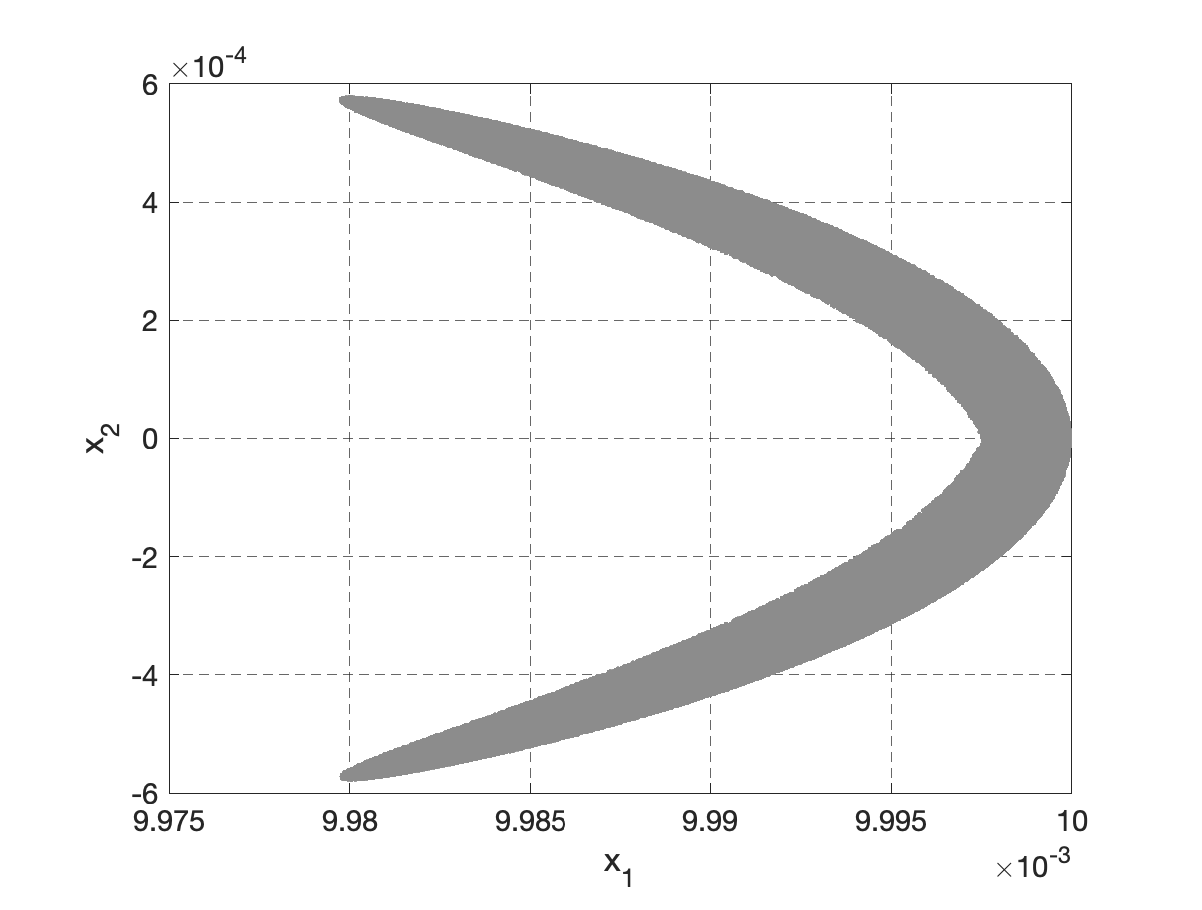
\includegraphics[width=\linewidth]{images/OsipovI_u=0_x1-x2.eps}
			%% This file was created by matlab2tikz.
%
%The latest updates can be retrieved from
%  http://www.mathworks.com/matlabcentral/fileexchange/22022-matlab2tikz-matlab2tikz
%where you can also make suggestions and rate matlab2tikz.
%
\begin{tikzpicture}
\node at (2.97,2.35) 
{
\includegraphics[width=0.985\linewidth]{images/OsipovI_u=0_x1-x2_1.eps}};
\pgfkeys{/pgf/number format/relative*={-3}}
\begin{axis}[%
width=0.761\linewidth,
height=0.6\linewidth,
at={(0\linewidth,0\linewidth)},
scale only axis,
xmin=0.009975,
xmax=0.01,
xlabel style={font=\color{white!15!black}},
xlabel={$ x_1 $},
ymin=-0.0006,
ymax=0.0006,
ylabel style={font=\color{white!15!black}},
ylabel={$ x_2 $},
xmajorgrids,
ymajorgrids,
grid style={dashed, opacity=0.7}
]
\end{axis}
\end{tikzpicture}%
			\subcaption{$ G_{x_1, x_2}(\varepsilon) $ системы \eqref{unicycle0};}
			\label{fig:u=0_x1-x2} 
		\end{minipage}
		\hfill
		\begin{minipage}[b]{.49\linewidth} 
			\small
			\centering
			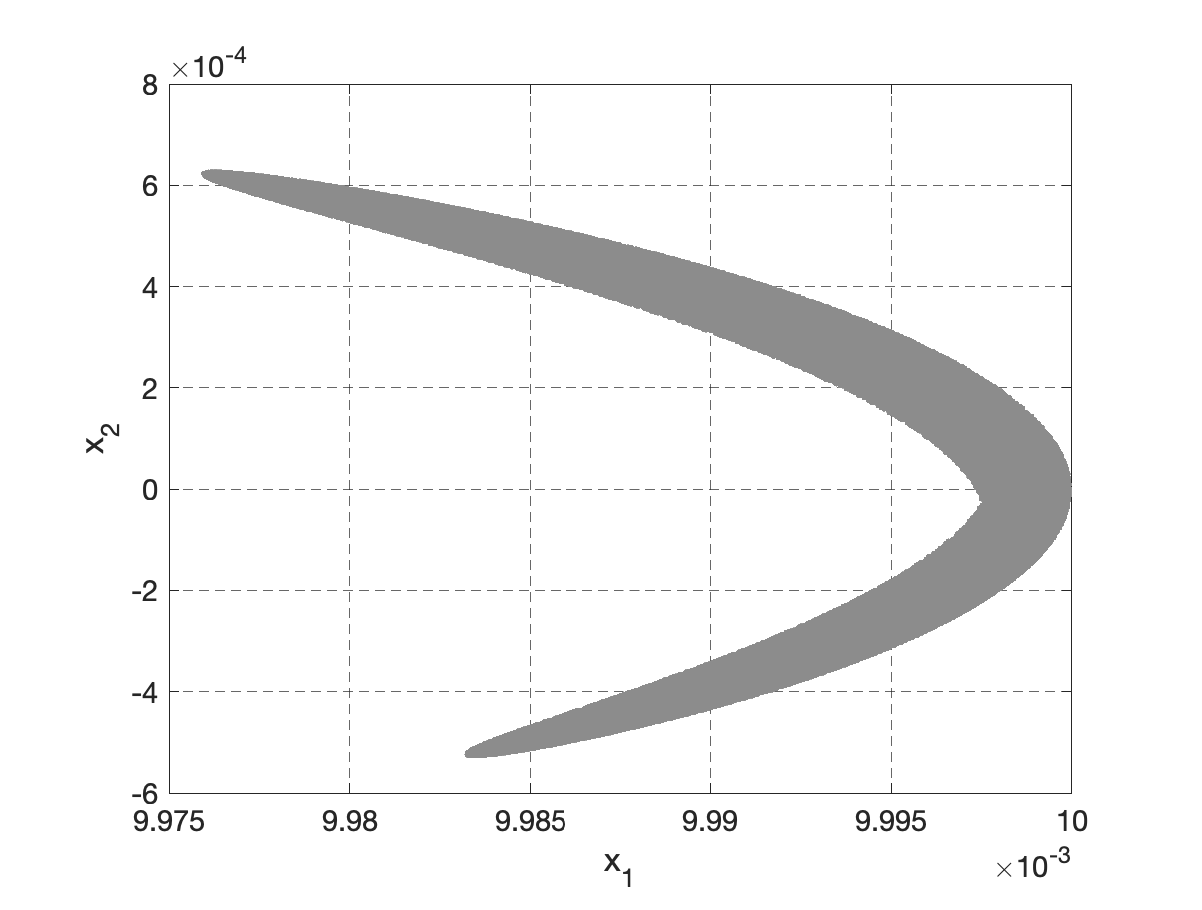
\includegraphics[width=\linewidth]{images/OsipovI_u=1_x1-x2.eps}
			%% This file was created by matlab2tikz.
%
%The latest updates can be retrieved from
%  http://www.mathworks.com/matlabcentral/fileexchange/22022-matlab2tikz-matlab2tikz
%where you can also make suggestions and rate matlab2tikz.
%
\begin{tikzpicture}
\node at (2.97,2.35) 
{
\includegraphics[width=0.985\linewidth]{OsipovI_u=1_x1-x2_1}};
\pgfkeys{/pgf/number format/relative*={-3}}
\begin{axis}[%
width=0.761\linewidth,
height=0.6\linewidth,
at={(0\linewidth,0\linewidth)},
scale only axis,
xmin=0.009975,
xmax=0.01,
xlabel style={font=\color{white!15!black}},
xlabel={$ x_1 $},
ymin=-0.0006,
ymax=0.0008,
ylabel style={font=\color{white!15!black}},
ylabel={$ x_2 $},
xmajorgrids,
ymajorgrids,
grid style={dashed, opacity=0.9}
]
\end{axis}
\end{tikzpicture}%
			\subcaption{$ G_{x_1, x_2}(\varepsilon) $ системы \eqref{unicycle1};}
			\label{fig:u=1_x1-x2}  
		\end{minipage} 
		\vfill
		\hspace{-2.5ex}
		\begin{minipage}[b]{.49\linewidth} 
			\small
			\centering 
			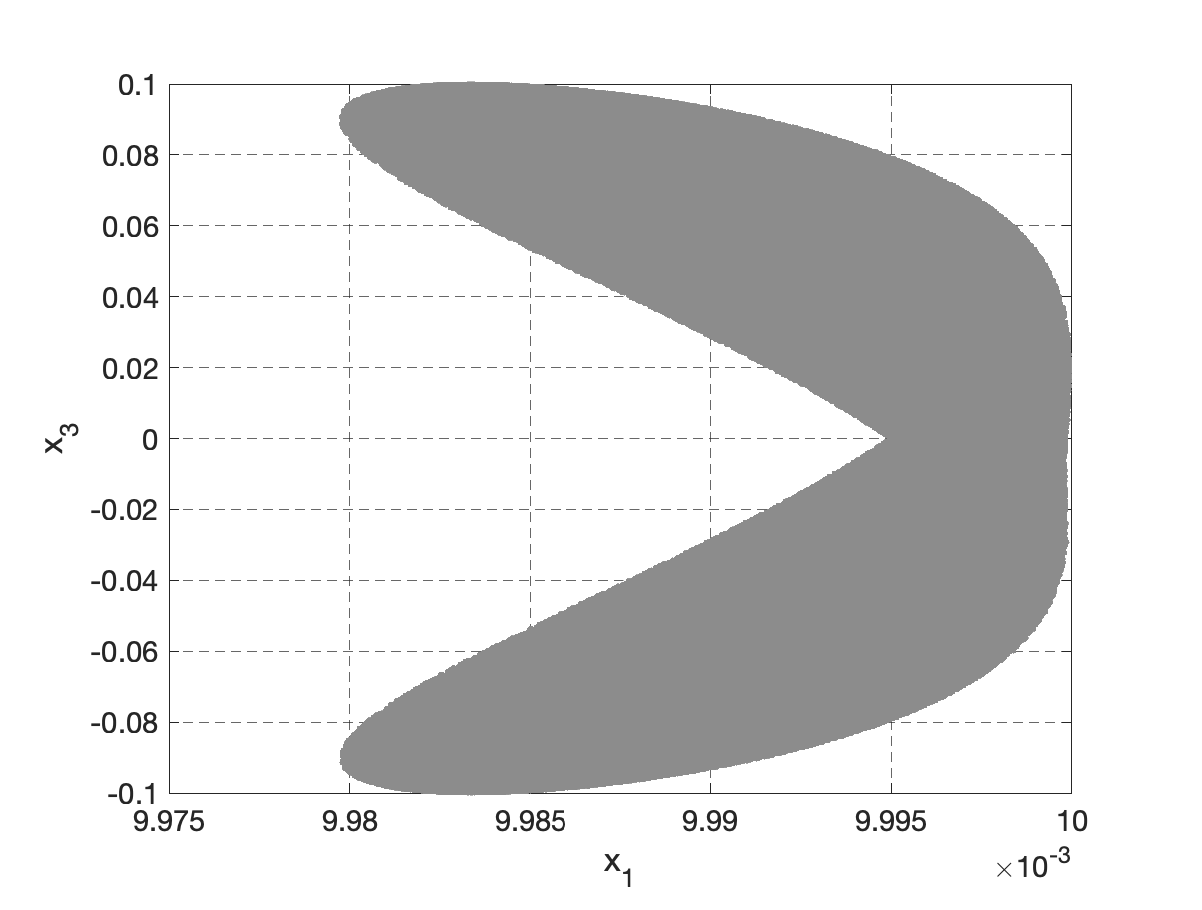
\includegraphics[width=\linewidth]{images/OsipovI_u=0_x1-x3.eps}
			%% This file was created by matlab2tikz.
%
%The latest updates can be retrieved from
%  http://www.mathworks.com/matlabcentral/fileexchange/22022-matlab2tikz-matlab2tikz
%where you can also make suggestions and rate matlab2tikz.
%
\begin{tikzpicture}
\node at (2.97,2.35) 
{
\includegraphics[width=0.985\linewidth]{OsipovI_u=0_x1-x3_1}};
\pgfkeys{/pgf/number format/.cd,fixed relative,precision=3}
\begin{axis}[%
width=0.761\linewidth,
height=0.6\linewidth,
at={(0\linewidth,0\linewidth)},
scale only axis,
xmin=0.009975,
xmax=0.01,
xlabel style={font=\color{white!15!black}},
ylabel near ticks,
xlabel={$ x_1 $},
ymin=-0.1,
ymax=0.1,
ylabel style={font=\color{white!15!black}},
ylabel={$ x_3 $},
xmajorgrids,
ymajorgrids,
grid style={dashed, opacity=0.7}
]
\end{axis}
\end{tikzpicture}%
			\subcaption{$ G_{x_1, x_3}(\varepsilon) $ системы \eqref{unicycle0};}
			\label{fig:u=0_x1-x3} 
		\end{minipage}
		\hfill
		\begin{minipage}[b]{.49\linewidth} 
			\small
			\centering
			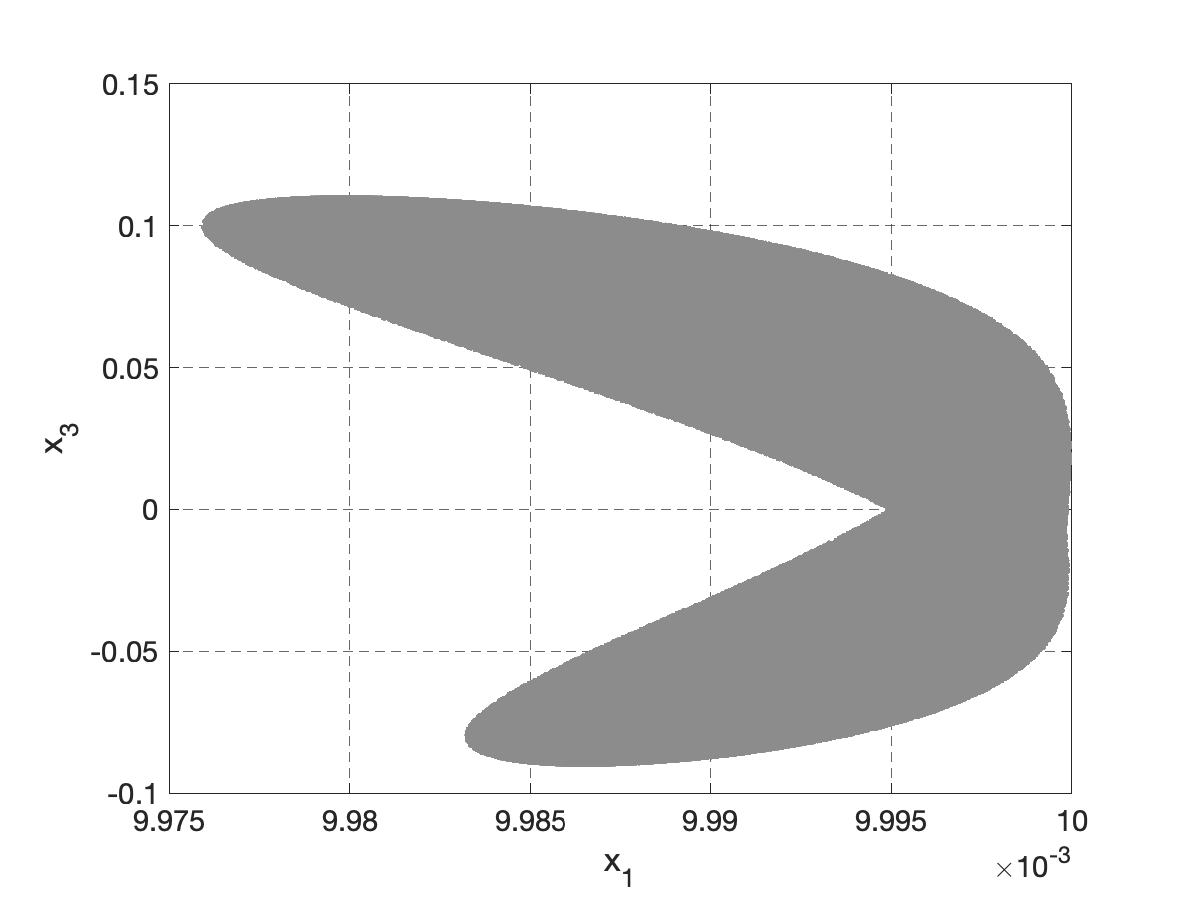
\includegraphics[width=\linewidth]{images/OsipovI_u=1_x1-x3.eps}
			%% This file was created by matlab2tikz.
%
%The latest updates can be retrieved from
%  http://www.mathworks.com/matlabcentral/fileexchange/22022-matlab2tikz-matlab2tikz
%where you can also make suggestions and rate matlab2tikz.
%
\begin{tikzpicture}
	
\node at (2.97,2.35) 
{
\includegraphics[width=0.985\linewidth]{OsipovI_u=1_x1-x3_1}};
\pgfkeys{/pgf/number format/relative*={-3}}

\begin{axis}[%
width=0.761\linewidth,
height=0.6\linewidth,
at={(0\linewidth,0\linewidth)},
scale only axis,
xmin=0.009975,
xmax=0.01,
xlabel style={font=\color{white!15!black}},
xlabel={$ x_1 $},
ymin=-0.1,
ymax=0.15,
ylabel style={font=\color{white!15!black}},
ylabel={$ x_3 $},
xmajorgrids,
ymajorgrids,
grid style={dashed, opacity=0.9}
]
\end{axis}
\end{tikzpicture}%
			\subcaption{$ G_{x_1, x_3}(\varepsilon) $ системы \eqref{unicycle1};}
			\label{fig:u=1_x1-x3}  
		\end{minipage} 
		\vfill
		\hspace{-2.5ex}
		\begin{minipage}[b]{.49\linewidth} 
			\small
			\centering 
			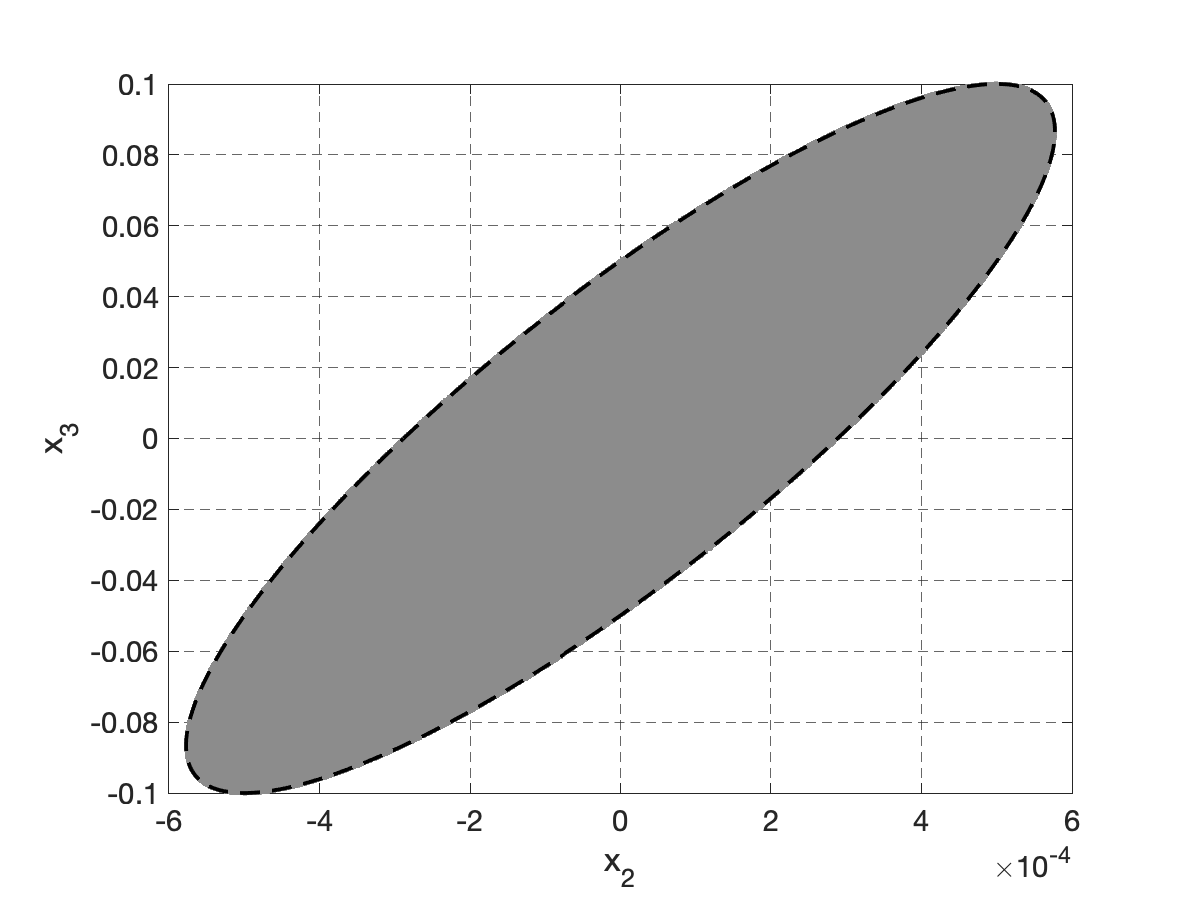
\includegraphics[width=\linewidth]{images/OsipovI_u=0_x2-x3.eps}
			%% This file was created by matlab2tikz.
%
%The latest updates can be retrieved from
%  http://www.mathworks.com/matlabcentral/fileexchange/22022-matlab2tikz-matlab2tikz
%where you can also make suggestions and rate matlab2tikz.
%
\begin{tikzpicture}
\node at (2.97,2.35) 
{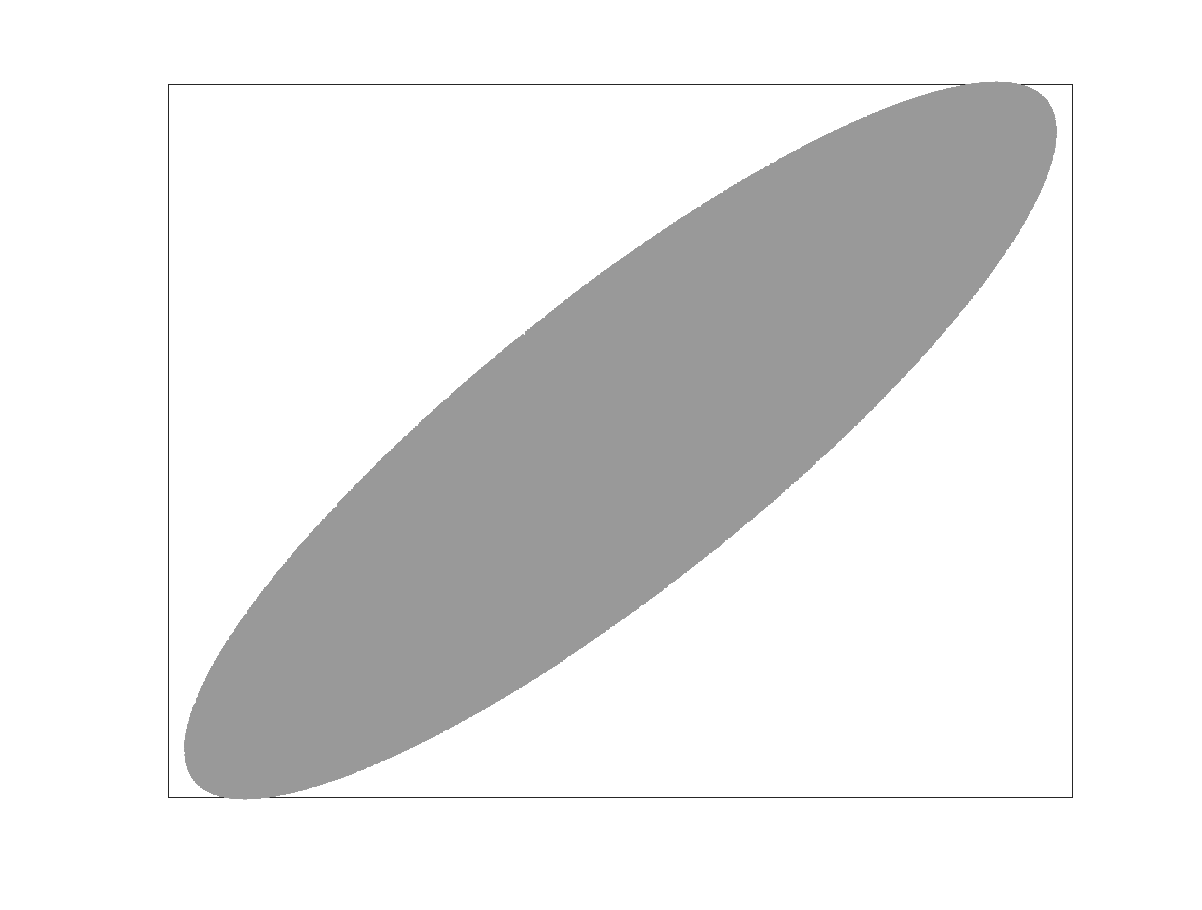
\includegraphics[width=0.985\linewidth]{OsipovI_u=0_x2-x3_1}};
\pgfkeys{/pgf/number format/.cd,fixed relative,precision=3}
\begin{axis}[%
width=0.761\linewidth,
height=0.6\linewidth,
at={(0\linewidth,0\linewidth)},
scale only axis,
xmin=-0.0006,
xmax=0.0006,
xlabel style={font=\color{white!15!black}},
xlabel={$ x_2 $},
ymin=-0.1,
ymax=0.1,
ylabel style={font=\color{white!15!black}},
ylabel={$ x_3 $},
xmajorgrids,
ymajorgrids,
grid style={dashed, opacity=0.7}
]
\addplot [color=black, dashed, line width=1.8pt, forget plot]
  table[row sep=crcr]{%
-0.00028866791780666	1.44335161666275e-06\\
-0.000279897676349703	0.00174668377533378\\
-0.0002710421753491	0.00349139214225243\\
-0.000262104112276241	0.00523503699730267\\
-0.000253086209751723	0.00697708720937059\\
-0.000243991214716013	0.00871701213308598\\
-0.000234821897592705	0.010454281770462\\
-0.00022558105144462	0.0121883669323379\\
-0.000216271491123012	0.0139187393995748\\
-0.000206896052410138	0.0156448720839568\\
-0.000197457591155454	0.0173662391887467\\
-0.000187958982405689	0.0190823163688491\\
-0.000178403119529083	0.0207925808905311\\
-0.00016879291333404	0.0224965117906516\\
-0.000159131291182461	0.024193590035352\\
-0.000149421196098048	0.0258832986781591\\
-0.000139665585869829	0.0275651230174517\\
-0.000129867432151182	0.0292385507532438\\
-0.000120029719554648	0.0309030721432363\\
-0.000110155444742784	0.0325581801580891\\
-0.000100247615515351	0.0342033706358677\\
-9.03092498931122e-05	0.035838142435615\\
-8.03433751985104e-05	0.0374619975900046\\
-7.03530271335194e-05	0.0390744414570258\\
-6.03412488549384e-05	0.0406749828706565\\
-5.03110900474174e-05	0.0422631342904774\\
-4.02656059944935e-05	0.0438384119501813\\
-3.02078566479219e-05	0.0454003360049329\\
-2.01409056955853e-05	0.0469484306775345\\
-1.00678196282645e-05	0.048482224403352\\
8.33319444416662e-09	0.0500012499739585\\
1.00844834787811e-05	0.0515050446794498\\
2.01575619317598e-05	0.0529931504493913\\
3.02245001961034e-05	0.0544651139923497\\
4.02822317848961e-05	0.0559204869339706\\
5.03276930156642e-05	0.0573588259535575\\
6.03578239436045e-05	0.0587796929191115\\
7.03695692936722e-05	0.0601826550207907\\
8.03598793912477e-05	0.0615672849027481\\
9.0325711091097e-05	0.0629331607933084\\
0.000100264028704343	0.0642798666334439\\
0.000110171804923167	0.0656069922035097\\
0.000120046021742952	0.0669141332482012\\
0.000129883671381603	0.0682008915996935\\
0.000139681757195739	0.0694668752989277\\
0.000149437294593506	0.0707116987150051\\
0.000159147311943709	0.0719349826626543\\
0.000168808851480998	0.0731363545177346\\
0.000178418970206839	0.074315448330741\\
0.000187974740785971	0.075471904938276\\
0.000197473252438107	0.076605372072454\\
0.000206911611824585	0.0777155044682059\\
0.000216286943929703	0.0788019639684498\\
0.000225596392936481	0.079864419627097\\
0.00023483712309657	0.0809025478098619\\
0.000244006319594044	0.0819160322928433\\
0.000253101189402829	0.0829045643588499\\
0.000262118962137475	0.0838678428914382\\
0.00027105689089705	0.0848055744666358\\
0.000279912253101871	0.0857174734423208\\
0.000288682351322827	0.0866032620452314\\
0.000297364514103041	0.0874626704555784\\
0.000305956096771624	0.0882954368892348\\
0.000314454482249267	0.0891013076774775\\
0.000322857081845429	0.089880037344258\\
0.000331161336046873	0.0906313886809759\\
0.000339364715297326	0.0913551328187356\\
0.000347464720767999	0.0920510492980618\\
0.00035545888511876	0.0927189261360531\\
0.000363344773249706	0.0933585598909551\\
0.000371119983042921	0.0939697557241295\\
0.00037878214609418	0.0945523274594049\\
0.000386328928434395	0.0951060976397873\\
0.000393758031240555	0.0956308975815151\\
0.000401067191535981	0.0961265674254422\\
0.000408254182879639	0.0965929561857326\\
0.000415316816044345	0.0970299217958519\\
0.00042225293968362	0.0974373311518421\\
0.000429060440987011	0.0978150601528669\\
0.000435737246323675	0.0981629937390134\\
0.000442281321874028	0.0984810259263407\\
0.000448690674249263	0.0987690598391637\\
0.000454963351098557	0.0990270077395624\\
0.000461097441703777	0.0992547910541074\\
0.000467091077561503	0.0994523403977945\\
0.000472942432952192	0.0996195955951801\\
0.000478649725496306	0.0997565056987106\\
0.000484211216697251	0.0998630290042424\\
0.00048962521247093	0.0999391330637446\\
0.000494890063661785	0.0999847946951835\\
0.00050000416654514	0.0999999999895837\\
0.000504965963315717	0.0999847443152654\\
0.000509773942562153	0.0999390323192546\\
0.000514426639727393	0.0998628779258683\\
0.00051892263755481	0.0997563043324723\\
0.000523260566519911	0.0996193440024157\\
0.00052743910524751	0.0994520386551416\\
0.000531456980914235	0.0992544392534797\\
0.000535312969636233	0.0990266059881218\\
0.000539005896841987	0.0987686082592877\\
0.000542534637630095	0.0984805246555848\\
0.000545898117111931	0.0981624429300695\\
0.00054909531073906	0.0978144599735168\\
0.000552125244615333	0.0974366817849062\\
0.000554986995793538	0.0970292234391336\\
0.000557679692556545	0.0965922090519583\\
0.000560202514682834	0.096125771742196\\
0.000562554693696348	0.0956300535911697\\
0.000564735513100572	0.0951052055994304\\
0.000566744308596789	0.0945513876407608\\
0.000568580468286433	0.0939687684134759\\
0.000570243432857474	0.0933575253890364\\
0.000571732695754795	0.0927178447579887\\
0.000573047803334489	0.0920499213732498\\
0.00057418835500205	0.091353958690753\\
0.000575154003334389	0.0906301687074733\\
0.00057594445418567	0.0898787718968512\\
0.000576559466776908	0.089099997141634\\
0.000576998853769308	0.0882940816641565\\
0.000577262481321336	0.0874612709540801\\
0.000577350269129487	0.0866018186936147\\
0.000577262190452743	0.0857159866802446\\
0.000576998272120724	0.0848040447469823\\
0.000576558594525508	0.0838662706801749\\
0.000575943291597151	0.0829029501348874\\
0.000575152550762886	0.08191437654789\\
0.000574186612890031	0.0809008510482736\\
0.000573045772212619	0.0798626823657238\\
0.000571730376241771	0.0788001867364783\\
0.000570240825659844	0.0777136878069983\\
0.000568577574198374	0.0766035165353828\\
0.000566741128499869	0.0754700110905558\\
0.000564732047963478	0.0743135167492561\\
0.000562550944574595	0.0731343857908635\\
0.000560198482718441	0.0719329773900902\\
0.000557675378977687	0.0707096575075735\\
0.000554982401914173	0.0694647987784002\\
0.000552120371834802	0.0681987803985984\\
0.000549090160541659	0.0669119880096307\\
0.000545892691066459	0.0656048135809243\\
0.000542528937389379	0.064277655290473\\
0.000538999924142375	0.0629309174035487\\
0.000535306726297067	0.0615650101495577\\
0.000531450468837296	0.0601803495970816\\
0.000527432326416442	0.058777357527138\\
0.000523253522999609	0.0573564613047026\\
0.0005189153314908	0.0559180937485293\\
0.000514419073345173	0.0544626929993095\\
0.000509766118166516	0.0529907023862101\\
0.000504957883290049	0.0515025702918314\\
0.000499995833350696	0.0499987500156252\\
0.000494881479836936	0.0484796996358155\\
0.000489616380630393	0.0469458818698633\\
0.00048420213953129	0.0453977639335186\\
0.000478640405769914	0.0438358173985018\\
0.000472932873504246	0.0422605180488582\\
0.000467081281303906	0.0406723457360301\\
0.000461087411620562	0.039071784232689\\
0.000454953090244985	0.0374593210853737\\
0.00044868018575089	0.0358354474659793\\
0.000442270608925752	0.0342006580221409\\
0.000435726312188764	0.0325554507265598\\
0.000429049288996108	0.0309003267253156\\
0.00042224157323373	0.0292357901852127\\
0.000415305238597798	0.0275623481402059\\
0.000408242397963038	0.0258805103369532\\
0.000401055202739125	0.0241907890795417\\
0.000393745842215349	0.0224936990734351\\
0.000386316542893733	0.0207897572686894\\
0.000378769567810818	0.0190794827024848\\
0.000371107215848326	0.0173633963410218\\
0.000363331821032889	0.0156420209208305\\
0.000355445751825092	0.0139158807895389\\
0.000347451410398008	0.0121855017461527\\
0.00033935123190548	0.0104514108808911\\
0.000331147683740344	0.00871413641462997\\
0.000322843264782841	0.00697420753800126\\
0.000314440504639433	0.0052321542501958\\
0.000305941962872257	0.00348850719752072\\
0.000297350228219465	0.00174379751175934\\
0.00028866791780666	-1.44335161666275e-06\\
0.000279897676349703	-0.00174668377533378\\
0.0002710421753491	-0.00349139214225243\\
0.000262104112276241	-0.00523503699730267\\
0.000253086209751723	-0.00697708720937059\\
0.000243991214716013	-0.00871701213308598\\
0.000234821897592705	-0.010454281770462\\
0.00022558105144462	-0.0121883669323379\\
0.000216271491123012	-0.0139187393995748\\
0.000206896052410138	-0.0156448720839568\\
0.000197457591155454	-0.0173662391887467\\
0.000187958982405689	-0.0190823163688491\\
0.000178403119529083	-0.0207925808905311\\
0.00016879291333404	-0.0224965117906516\\
0.000159131291182461	-0.024193590035352\\
0.000149421196098048	-0.0258832986781591\\
0.000139665585869829	-0.0275651230174517\\
0.000129867432151182	-0.0292385507532438\\
0.000120029719554648	-0.0309030721432363\\
0.000110155444742784	-0.0325581801580891\\
0.000100247615515351	-0.0342033706358677\\
9.03092498931122e-05	-0.035838142435615\\
8.03433751985104e-05	-0.0374619975900046\\
7.03530271335194e-05	-0.0390744414570258\\
6.03412488549384e-05	-0.0406749828706565\\
5.03110900474174e-05	-0.0422631342904774\\
4.02656059944935e-05	-0.0438384119501813\\
3.02078566479219e-05	-0.0454003360049329\\
2.01409056955853e-05	-0.0469484306775345\\
1.00678196282645e-05	-0.048482224403352\\
-8.33319444416662e-09	-0.0500012499739585\\
-1.00844834787811e-05	-0.0515050446794498\\
-2.01575619317598e-05	-0.0529931504493913\\
-3.02245001961034e-05	-0.0544651139923497\\
-4.02822317848961e-05	-0.0559204869339706\\
-5.03276930156642e-05	-0.0573588259535575\\
-6.03578239436045e-05	-0.0587796929191115\\
-7.03695692936722e-05	-0.0601826550207907\\
-8.03598793912477e-05	-0.0615672849027481\\
-9.0325711091097e-05	-0.0629331607933084\\
-0.000100264028704343	-0.0642798666334439\\
-0.000110171804923167	-0.0656069922035097\\
-0.000120046021742952	-0.0669141332482012\\
-0.000129883671381603	-0.0682008915996935\\
-0.000139681757195739	-0.0694668752989277\\
-0.000149437294593506	-0.0707116987150051\\
-0.000159147311943709	-0.0719349826626543\\
-0.000168808851480998	-0.0731363545177346\\
-0.000178418970206839	-0.074315448330741\\
-0.000187974740785971	-0.075471904938276\\
-0.000197473252438107	-0.076605372072454\\
-0.000206911611824585	-0.0777155044682059\\
-0.000216286943929703	-0.0788019639684498\\
-0.000225596392936481	-0.079864419627097\\
-0.00023483712309657	-0.0809025478098619\\
-0.000244006319594044	-0.0819160322928433\\
-0.000253101189402829	-0.0829045643588499\\
-0.000262118962137475	-0.0838678428914382\\
-0.00027105689089705	-0.0848055744666358\\
-0.000279912253101871	-0.0857174734423208\\
-0.000288682351322827	-0.0866032620452314\\
-0.000297364514103041	-0.0874626704555784\\
-0.000305956096771624	-0.0882954368892348\\
-0.000314454482249267	-0.0891013076774775\\
-0.000322857081845429	-0.089880037344258\\
-0.000331161336046873	-0.0906313886809759\\
-0.000339364715297326	-0.0913551328187356\\
-0.000347464720767999	-0.0920510492980618\\
-0.00035545888511876	-0.0927189261360531\\
-0.000363344773249706	-0.0933585598909551\\
-0.000371119983042921	-0.0939697557241295\\
-0.00037878214609418	-0.0945523274594049\\
-0.000386328928434395	-0.0951060976397873\\
-0.000393758031240555	-0.0956308975815151\\
-0.000401067191535981	-0.0961265674254422\\
-0.000408254182879639	-0.0965929561857326\\
-0.000415316816044345	-0.0970299217958519\\
-0.00042225293968362	-0.0974373311518421\\
-0.000429060440987011	-0.0978150601528669\\
-0.000435737246323675	-0.0981629937390134\\
-0.000442281321874028	-0.0984810259263407\\
-0.000448690674249263	-0.0987690598391637\\
-0.000454963351098557	-0.0990270077395624\\
-0.000461097441703777	-0.0992547910541074\\
-0.000467091077561503	-0.0994523403977945\\
-0.000472942432952192	-0.0996195955951801\\
-0.000478649725496306	-0.0997565056987106\\
-0.000484211216697251	-0.0998630290042424\\
-0.00048962521247093	-0.0999391330637446\\
-0.000494890063661785	-0.0999847946951835\\
-0.00050000416654514	-0.0999999999895837\\
-0.000504965963315717	-0.0999847443152654\\
-0.000509773942562153	-0.0999390323192546\\
-0.000514426639727393	-0.0998628779258683\\
-0.00051892263755481	-0.0997563043324723\\
-0.000523260566519911	-0.0996193440024157\\
-0.00052743910524751	-0.0994520386551416\\
-0.000531456980914235	-0.0992544392534797\\
-0.000535312969636233	-0.0990266059881218\\
-0.000539005896841987	-0.0987686082592877\\
-0.000542534637630095	-0.0984805246555848\\
-0.000545898117111931	-0.0981624429300695\\
-0.00054909531073906	-0.0978144599735168\\
-0.000552125244615333	-0.0974366817849062\\
-0.000554986995793538	-0.0970292234391336\\
-0.000557679692556545	-0.0965922090519583\\
-0.000560202514682834	-0.096125771742196\\
-0.000562554693696348	-0.0956300535911697\\
-0.000564735513100572	-0.0951052055994304\\
-0.000566744308596789	-0.0945513876407608\\
-0.000568580468286433	-0.0939687684134759\\
-0.000570243432857474	-0.0933575253890364\\
-0.000571732695754795	-0.0927178447579887\\
-0.000573047803334489	-0.0920499213732498\\
-0.00057418835500205	-0.091353958690753\\
-0.000575154003334389	-0.0906301687074733\\
-0.00057594445418567	-0.0898787718968512\\
-0.000576559466776908	-0.089099997141634\\
-0.000576998853769308	-0.0882940816641565\\
-0.000577262481321336	-0.0874612709540801\\
-0.000577350269129487	-0.0866018186936147\\
-0.000577262190452743	-0.0857159866802446\\
-0.000576998272120724	-0.0848040447469823\\
-0.000576558594525508	-0.0838662706801749\\
-0.000575943291597151	-0.0829029501348874\\
-0.000575152550762886	-0.08191437654789\\
-0.000574186612890031	-0.0809008510482736\\
-0.000573045772212619	-0.0798626823657238\\
-0.000571730376241771	-0.0788001867364783\\
-0.000570240825659844	-0.0777136878069983\\
-0.000568577574198374	-0.0766035165353828\\
-0.000566741128499869	-0.0754700110905558\\
-0.000564732047963478	-0.0743135167492561\\
-0.000562550944574595	-0.0731343857908635\\
-0.000560198482718441	-0.0719329773900902\\
-0.000557675378977687	-0.0707096575075735\\
-0.000554982401914173	-0.0694647987784002\\
-0.000552120371834802	-0.0681987803985984\\
-0.000549090160541659	-0.0669119880096307\\
-0.000545892691066459	-0.0656048135809243\\
-0.000542528937389379	-0.064277655290473\\
-0.000538999924142375	-0.0629309174035487\\
-0.000535306726297067	-0.0615650101495577\\
-0.000531450468837296	-0.0601803495970816\\
-0.000527432326416442	-0.058777357527138\\
-0.000523253522999609	-0.0573564613047026\\
-0.0005189153314908	-0.0559180937485293\\
-0.000514419073345173	-0.0544626929993095\\
-0.000509766118166516	-0.0529907023862101\\
-0.000504957883290049	-0.0515025702918314\\
-0.000499995833350696	-0.0499987500156252\\
-0.000494881479836936	-0.0484796996358155\\
-0.000489616380630393	-0.0469458818698633\\
-0.00048420213953129	-0.0453977639335186\\
-0.000478640405769914	-0.0438358173985018\\
-0.000472932873504246	-0.0422605180488582\\
-0.000467081281303906	-0.0406723457360301\\
-0.000461087411620562	-0.039071784232689\\
-0.000454953090244985	-0.0374593210853737\\
-0.00044868018575089	-0.0358354474659793\\
-0.000442270608925752	-0.0342006580221409\\
-0.000435726312188764	-0.0325554507265598\\
-0.000429049288996108	-0.0309003267253156\\
-0.00042224157323373	-0.0292357901852127\\
-0.000415305238597798	-0.0275623481402059\\
-0.000408242397963038	-0.0258805103369532\\
-0.000401055202739125	-0.0241907890795417\\
-0.000393745842215349	-0.0224936990734351\\
-0.000386316542893733	-0.0207897572686894\\
-0.000378769567810818	-0.0190794827024848\\
-0.000371107215848326	-0.0173633963410218\\
-0.000363331821032889	-0.0156420209208305\\
-0.000355445751825092	-0.0139158807895389\\
-0.000347451410398008	-0.0121855017461527\\
-0.00033935123190548	-0.0104514108808911\\
-0.000331147683740344	-0.00871413641462997\\
-0.000322843264782841	-0.00697420753800126\\
-0.000314440504639433	-0.0052321542501958\\
-0.000305941962872257	-0.00348850719752072\\
-0.000297350228219465	-0.00174379751175934\\
-0.00028866791780666	1.44335161666275e-06\\
};
\end{axis}
\end{tikzpicture}%
			\subcaption{$ G_{x_2, x_3}(\varepsilon) $ системы \eqref{unicycle0};}
			\label{fig:u=0_x2-x3} 
		\end{minipage}
		\hfill
		\begin{minipage}[b]{.49\linewidth} 
			\small
			\centering
			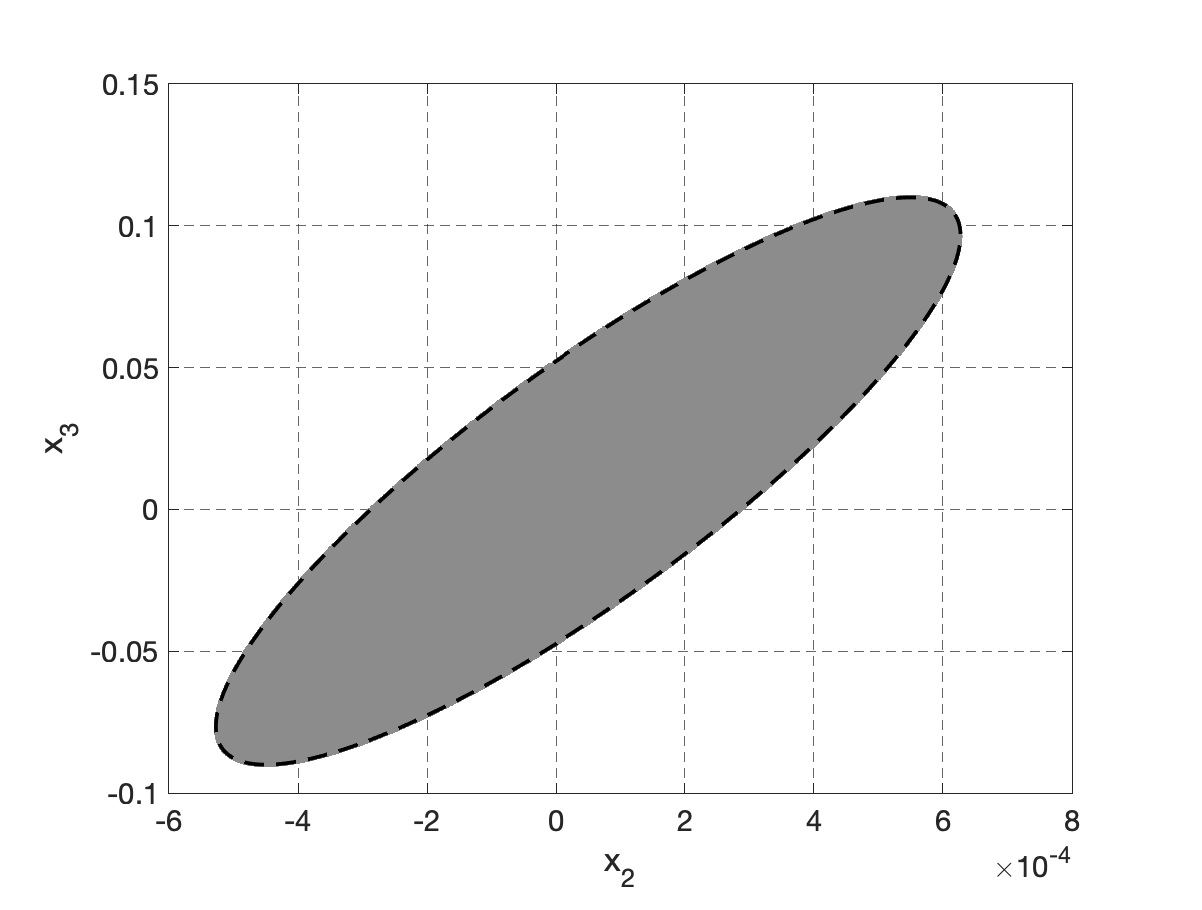
\includegraphics[width=\linewidth]{images/OsipovI_u=1_x2-x3.eps}
			%% This file was created by matlab2tikz.
%
%The latest updates can be retrieved from
%  http://www.mathworks.com/matlabcentral/fileexchange/22022-matlab2tikz-matlab2tikz
%where you can also make suggestions and rate matlab2tikz.
%
\begin{tikzpicture}
\node at (2.97,2.35) 
{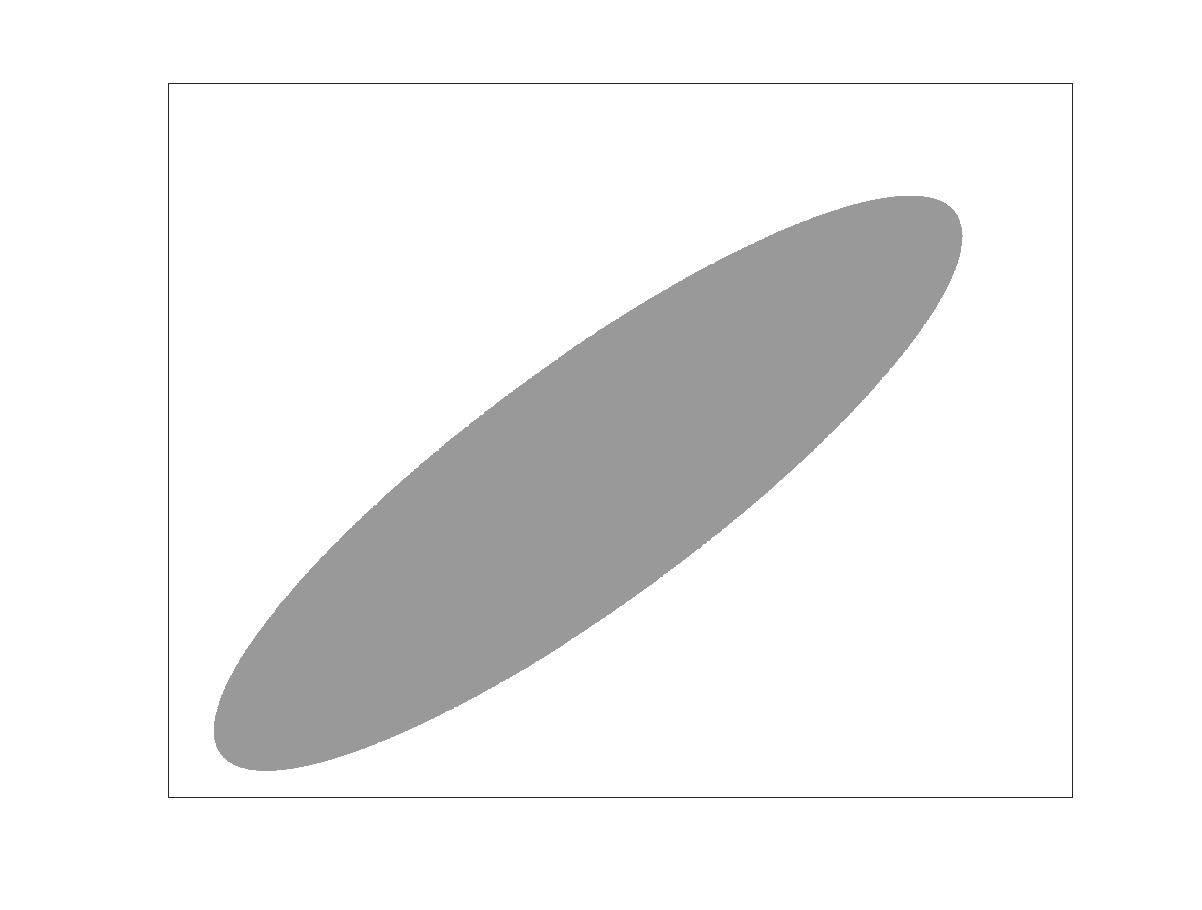
\includegraphics[width=0.985\linewidth]{OsipovI_u=1_x2-x3_1}};
\begin{axis}[%
width=0.761\linewidth,
height=0.6\linewidth,
at={(0\linewidth,0\linewidth)},
scale only axis,
xmin=-0.0006,
xmax=0.0008,
xlabel style={font=\color{white!15!black}},
xlabel={$ x_2 $},
ymin=-0.1,
ymax=0.15,
ylabel style={font=\color{white!15!black}},
ylabel={$ x_3 $},
xmajorgrids,
ymajorgrids,
grid style={dashed, opacity=0.9}
]
\addplot [color=black, dashed, line width=1.8pt, forget plot]
  table[row sep=crcr]{%
-0.000238655344918043	0.0100014432505853\\
-0.000212092211410247	0.0152350368964098\\
-0.000184810702510835	0.0204542816699843\\
-0.000156885594939385	0.0256448719841695\\
-0.000128393429474696	0.0307925807917078\\
-9.94123011618386e-05	0.0358832985805707\\
-7.00216452590718e-05	0.0409030720471502\\
-4.03020195113013e-05	0.0458381423412946\\
-1.03348833469241e-05	0.0506749827783604\\
1.97976253968335e-05	0.055400335914914\\
5.00129156079804e-05	0.0600012498864635\\
7.01615368250419e-05	0.0629931503637126\\
9.02855938074709e-05	0.0659204868502126\\
0.00011036056849173	0.0687796928373763\\
0.00013036200261346	0.0715672848231352\\
0.000150265527506188	0.0742798665560503\\
0.000170046893790729	0.0769141331731213\\
0.000189682000919345	0.0794668752262528\\
0.000209146926538575	0.081934982592473\\
0.000228417955634871	0.084315448263139\\
0.000247471609427757	0.0866053720075135\\
0.00026628467397509	0.0888019639062498\\
0.000284834228455641	0.0909025477504784\\
0.00030309767309461	0.0929045643023551\\
0.000321052756697984	0.0948055744130986\\
0.000338677603762161	0.096603261994717\\
0.000355950741125877	0.0982954368418047\\
0.00037285112413199	0.0998800372999701\\
0.000389358162267109	0.101355132777644\\
0.000405451744247984	0.102718926098207\\
0.00042111226252399	0.103969755689576\\
0.000436320637165935	0.105106097608568\\
0.000451058339111979	0.106126567397596\\
0.000458245053689743	0.106592956159585\\
0.000465307412742477	0.107029921771412\\
0.000472243265007194	0.107437331129116\\
0.000479050497756109	0.107815060131863\\
0.000485727037440181	0.108162993719737\\
0.000492270850320747	0.108481025908798\\
0.000498679943089012	0.10876905982336\\
0.000504952363473227	0.109027007725503\\
0.000511086200833386	0.109254791041796\\
0.000517079586743199	0.109452340387235\\
0.000522930695559282	0.109619595586376\\
0.00052863774497719	0.109756505691665\\
0.000534198996574392	0.109863028998956\\
0.000539612756339777	0.10993913306022\\
0.00054487737518967	0.109984794693422\\
0.00054999124947018	0.109999999989585\\
0.000554952821445659	0.10998474431703\\
0.000559760579773208	0.109939032322782\\
0.00056441305996309	0.109862877931157\\
0.000568908844824745	0.109756304339521\\
0.000573246564898572	0.109619344011223\\
0.000577424898872997	0.109452038665704\\
0.000581442573987026	0.109254439265794\\
0.000585298366417908	0.109026606002184\\
0.000588991101653905	0.108768608275094\\
0.000592519654852089	0.10848052467313\\
0.000595882951180973	0.108162442949349\\
0.000599079966147928	0.107814459994524\\
0.000602109725911223	0.107436681807635\\
0.000604971307576668	0.107029223463577\\
0.000607663839478786	0.106592209078109\\
0.000610186501446258	0.106125771770045\\
0.000612538525051817	0.10563005362071\\
0.000616727843576859	0.104551387673655\\
0.000620226691014594	0.103357525425244\\
0.000623030804558375	0.102049921412727\\
0.000625136767827786	0.100630168750172\\
0.000626542015030984	0.0990999971875026\\
0.000627244834090712	0.0974612710030624\\
0.000627244368730212	0.0957159867322809\\
0.000626540619516447	0.0938662707352017\\
0.000625134443859435	0.0919143766058404\\
0.000623027554967598	0.0898626824265272\\
0.00062022251976053	0.0877136878705805\\
0.000616722755741525	0.0854700111568394\\
0.000612532526833964	0.0831343858597678\\
0.000607656938186305	0.0807096575790145\\
0.00060210192995229	0.078198780472489\\
0.000595874270053767	0.0756048136571746\\
0.000588981545935036	0.0729309174820657\\
0.000581432155318667	0.0701803496777697\\
0.000573235295974264	0.0673564613874635\\
0.000564400954512281	0.0644626930840423\\
0.000554939894216983	0.0615025703784329\\
0.000544863641932958	0.0584796997241802\\
0.00053418447402151	0.0553977640235389\\
0.00051706391371599	0.0506723458283275\\
0.000498663162546154	0.0458354475603007\\
0.000479032655691922	0.0409003268214026\\
0.00045822619900808	0.0358805104345424\\
0.000436300821546165	0.0307897573675133\\
0.00041331661924178	0.0256420210206182\\
0.000389336590195827	0.0204514109813691\\
0.000364426462001091	0.0152321543510888\\
0.000338654511587488	0.0099985567494147\\
0.000312091378079693	0.00476496310359015\\
0.00028480986918028	-0.000454281669984291\\
0.00025688476160883	-0.00564487198416951\\
0.000228392596144142	-0.0107925807917078\\
0.000199411467831284	-0.0158832985805707\\
0.000170020811928517	-0.0209030720471502\\
0.000140301186180747	-0.0258381423412947\\
0.00011033405001637	-0.0306749827783604\\
8.0201541272612e-05	-0.035400335914914\\
4.99862510614513e-05	-0.0400012498864635\\
2.98376298444036e-05	-0.0429931503637126\\
9.71357286197461e-06	-0.0459204868502126\\
-1.03614018222842e-05	-0.0487796928373763\\
-3.03628359440145e-05	-0.0515672848231352\\
-5.02663608367426e-05	-0.0542798665560503\\
-7.00477271212835e-05	-0.0569141331731213\\
-8.96828342499129e-05	-0.0594668752262528\\
-0.00010914775986913	-0.0619349825924731\\
-0.000128418788965426	-0.064315448263139\\
-0.000147472442758312	-0.0666053720075135\\
-0.000166285507305644	-0.0688019639062498\\
-0.000184835061786195	-0.0709025477504784\\
-0.000203098506425164	-0.0729045643023551\\
-0.000221053590028539	-0.0748055744130986\\
-0.000238678437092715	-0.076603261994717\\
-0.000255951574456431	-0.0782954368418047\\
-0.000272851957462544	-0.0798800372999701\\
-0.000289358995597663	-0.0813551327776438\\
-0.000305452577578538	-0.0827189260982075\\
-0.000321113095854544	-0.0839697556895761\\
-0.00033632147049649	-0.0851060976085683\\
-0.000351059172442533	-0.0861265673975956\\
-0.000358245887020298	-0.0865929561595852\\
-0.000365308246073032	-0.0870299217714116\\
-0.000372244098337748	-0.0874373311291165\\
-0.000379051331086663	-0.0878150601318628\\
-0.000385727870770736	-0.0881629937197372\\
-0.000392271683651302	-0.0884810259087982\\
-0.000398680776419566	-0.0887690598233604\\
-0.000404953196803781	-0.089027007725503\\
-0.00041108703416394	-0.0892547910417962\\
-0.000417080420073754	-0.0894523403872353\\
-0.000422931528889836	-0.0896195955863761\\
-0.000428638578307744	-0.0897565056916645\\
-0.000434199829904947	-0.0898630289989563\\
-0.000439613589670332	-0.0899391330602201\\
-0.000444878208520225	-0.0899847946934217\\
-0.000449992082800735	-0.0899999999895852\\
-0.000454953654776213	-0.0899847443170301\\
-0.000459761413103763	-0.089939032322782\\
-0.000464413893293644	-0.0898628779311573\\
-0.000468909678155299	-0.0897563043395214\\
-0.000473247398229126	-0.0896193440112226\\
-0.000477425732203551	-0.0894520386657038\\
-0.000481443407317581	-0.0892544392657938\\
-0.000485299199748462	-0.0890266060021841\\
-0.000488991934984459	-0.0887686082750939\\
-0.000492520488182643	-0.0884805246731301\\
-0.000495883784511528	-0.0881624429493486\\
-0.000499080799478482	-0.0878144599945238\\
-0.000502110559241778	-0.0874366818076348\\
-0.000504972140907223	-0.0870292234635768\\
-0.000507664672809341	-0.0865922090781085\\
-0.000510187334776813	-0.0861257717700454\\
-0.000512539358382372	-0.0856300536207098\\
-0.000516728676907427	-0.0845513876736548\\
-0.000520227524345149	-0.0833575254252442\\
-0.000523031637888929	-0.0820499214127272\\
-0.00052513760115834	-0.0806301687501723\\
-0.000526542848361539	-0.0790999971875026\\
-0.000527245667421267	-0.0774612710030624\\
-0.000527245202060767	-0.0757159867322809\\
-0.000526541452847001	-0.0738662707352017\\
-0.000525135277189989	-0.0719143766058404\\
-0.000523028388298152	-0.0698626824265272\\
-0.000520223353091084	-0.0677136878705805\\
-0.000516723589072079	-0.0654700111568394\\
-0.000512533360164519	-0.0631343858597678\\
-0.000507657771516859	-0.0607096575790145\\
-0.000502102763282844	-0.058198780472489\\
-0.000495875103384322	-0.0556048136571746\\
-0.00048898237926559	-0.0529309174820657\\
-0.000481432988649222	-0.0501803496777697\\
-0.000473236129304819	-0.0473564613874635\\
-0.000464401787842836	-0.0444626930840423\\
-0.000454940727547537	-0.0415025703784329\\
-0.000444864475263512	-0.0384796997241802\\
-0.000434185307352064	-0.0353977640235389\\
-0.000417064747046544	-0.0306723458283275\\
-0.000398663995876708	-0.0258354475603007\\
-0.000379033489022476	-0.0209003268214026\\
-0.000358227032338634	-0.0158805104345424\\
-0.000336301654876719	-0.0107897573675133\\
-0.000313317452572334	-0.00564202102061818\\
-0.000289337423526381	-0.00045141098136911\\
-0.000264427295331646	0.00476784564891122\\
-0.000238655344918043	0.0100014432505853\\
};
\end{axis}
\end{tikzpicture}%
			\subcaption{$ G_{x_2, x_3}(\varepsilon) $ системы \eqref{unicycle1};}
			\label{fig:u=1_x2-x3}  
		\end{minipage}
		\caption{Результаты численного эксперимента для $ \varepsilon = 0.01 $.}\label{fig:RS}
	\end{figure}
	
	Немного изменим рассмотренный пример для того, чтобы линеаризованная система оставалась управляемой. Итак, рассматривается нелинейная система
	\begin{equation}\label{unicycle1}
		\dot{x_1} = \cos(x_3), \qquad
		\dot{x_2} = \sin(x_3), \qquad
		\dot{x_3} = 1 + u(t), \qquad 0 \leq t \leq \varepsilon
	\end{equation}
	при интегральных ограничениях на управление 
	\begin{equation*}
		\int_0^1 u^2(t) dt \leqslant 1
	\end{equation*}
	и нулевых начальных условиях $ x_1(0) = x_2(0) = x_3(0) = 0 $. Фактически, это то же самое, что рассматривать исходную систему при ограничении $ \displaystyle{\int_0^1} \left( u(t) - 1\right)^2 \ dt \leqslant 1$.
	
	Порождённое нулевым управлением $ u(t) \equiv 0 $ решение обозначим $ x(t,0) = x(t) $ и будем использовать его как опорное. 
	\begin{gather}\label{trj}
		\begin{gathered}
			\dot{x_3} = 1 \longrightarrow x_3(t) = x_3(0) + t = t, \\
			\dot{x_2} = \sin(x_3(t)) = \sin(t) \longrightarrow x_2(t) = x_2(0) + \int_0^t \sin(\tau) d\tau = 1 - \cos(t),\\
			\dot{x_1} = \cos(x_3(t)) = \cos(t) \longrightarrow x_1(t) = x_1(0) + \int_0^t \cos(\tau) d\tau = \sin(t).
		\end{gathered}
	\end{gather}
	Выпишем матрицы линеаризованной вдоль траектории \eqref{trj} системы 
	\begin{gather*}
		A(t) = \begin{pmatrix}
			0 & 0 & -\sin(t) \\ 
			0 & 0 & \cos(t) \\ 
			0 & 0 & 0
		\end{pmatrix}, \qquad  B = \begin{pmatrix}
			0 \\ 
			0 \\ 
			1
		\end{pmatrix}.
	\end{gather*}
	Для изучения грамиана управляемости выпишем фундаментальную матрицу линеаризованной системы
	\begin{gather*}
		\begin{gathered}
			X(t,\tau) = \begin{pmatrix}
				1 & 0 & \cos(t)-\cos(t_1) \\ 
				0 & 1 & \sin(t)-\sin(t_1) \\ 
				0 & 0 & 1
			\end{pmatrix}.
		\end{gathered}	
	\end{gather*}
	Грамиан управляемости имеет вид
	\begin{gather*}
		W(\varepsilon) = \int_0^{\varepsilon}X(\varepsilon,t) B B^{\top} X^{\top}(\varepsilon,t)dt =
	\end{gather*}
	\begin{gather*}
		=\begin{pmatrix}
			\varepsilon-\dfrac{3}{4} \sin(2\varepsilon) +\dfrac{1}{2}\varepsilon \cos(2\varepsilon)& \dfrac{3}{2}\cos^2(\varepsilon) - \cos(\varepsilon) + \dfrac{1}{2}\varepsilon \sin(2 \varepsilon) - \dfrac{1}{2} &  \varepsilon\cos( \varepsilon)-\sin( \varepsilon) \\[8pt] 
			* & \dfrac{3}{4}\sin(2\varepsilon) + \dfrac{1}{2}\varepsilon + \varepsilon \sin^2(\varepsilon) - 2 \sin(\varepsilon) & \cos(\varepsilon) + \varepsilon\sin(\varepsilon)-1 \\ 
			* & * & \varepsilon
		\end{pmatrix}.	
	\end{gather*}
	Здесь и далее, будем заменять элементы симметричных матриц под главной диагональю на $ * $ для лаконичной записи.
	Проделаем замену времени $ t = \varepsilon \tau $ и выпишем грамиан управляемости $ \widetilde{W}(\varepsilon) $ линеаризованной системы в новом времени $ \tau $
	\begin{gather*}
		\widetilde{W}(\varepsilon) = \dfrac{1}{\varepsilon} W(\varepsilon) = 
	\end{gather*} \footnotesize
	\begin{gather*}
		=\begin{pmatrix} 
			\cos^2(\varepsilon)-\dfrac{3}{4\varepsilon}\sin(2\varepsilon)+\dfrac{1}{2} & 
			\cos\left(\varepsilon \right)\,\sin\left(\varepsilon \right)+\dfrac{1}{2\,\varepsilon}\left( 3\cos^2\left(\varepsilon \right)-2\cos\left(\varepsilon\right)-1\right) &
			\cos\left(\varepsilon \right)-\dfrac{1}{\varepsilon} \sin\left(\varepsilon \right) \\[8pt] 
			* &
			\dfrac{3}{2}-\dfrac{2\,\sin\left(\varepsilon \right)-\dfrac{3\,\cos\left(\varepsilon \right)\,\sin\left(\varepsilon \right)}{2}}{\varepsilon }-{\cos\left(\varepsilon \right)}^2 & \sin\left(\varepsilon \right)+\dfrac{1}{\varepsilon } \left(\cos\left(\varepsilon \right)-1 \right)\\
			* &
			* & 
			1 \end{pmatrix}.	
	\end{gather*}
	\normalsize
	Далее последовательно рассмотрим проекции системы \eqref{unicycle1} на координатные плоскости $ (x_1, x_2) $, $ (x_1, x_3) $, $ (x_2, x_3) $. \\
	
	\begin{enumerate}
		\item Будем рассматривать проекцию $ G_{x_1, x_2}(\varepsilon) $ области достижимости системы \eqref{unicycle1} на плоскость первых двух фазовых координат. Матрица проектирования будет иметь вид
		\begin{equation*}
			C = \begin{pmatrix}
				1 & 0 & 0 \\ 
				0 & 1 & 0 
			\end{pmatrix}. 
		\end{equation*} 
		Тогда: \small
		\begin{equation}\label{Ve}
			\widetilde{W}_{x_1,x_2}(\varepsilon)= \begin{pmatrix}
				\cos^2(\varepsilon)-\dfrac{3}{4\varepsilon}\sin(2\varepsilon)+\dfrac{1}{2} & 
				\cos\left(\varepsilon \right)\,\sin\left(\varepsilon \right)+\dfrac{1}{2\,\varepsilon}\left( 3\cos^2\left(\varepsilon \right)-2\cos\left(\varepsilon\right)-1\right) \\[6pt]
				* &
				\dfrac{3}{2}-\dfrac{1}{\varepsilon }\left(2\,\sin\left(\varepsilon \right)-\dfrac{3\,\cos\left(\varepsilon \right)\,\sin\left(\varepsilon \right)}{2} \right) -{\cos\left(\varepsilon \right)}^2 
			\end{pmatrix}
		\end{equation}
		\normalsize
		Для исследования асимптотики $ \nu^{x_1,x_2}(\varepsilon) $ -- минимального собственного числа $ \widetilde{W}_{x_1,x_2}(\varepsilon) $, перепишем \eqref{Ve}, разложив тригонометрические функции в ряд вблизи точки $ \varepsilon = 0 $.
		\begin{gather*}
			\widetilde{W}_{x_1,x_2}(\varepsilon) = \begin{pmatrix}
				\dfrac{2\,\varepsilon ^4}{15} + O(\varepsilon^6)&
				-\dfrac{5\,\varepsilon ^3}{24} + O(\varepsilon^5)\\[8pt]
				-\dfrac{5\,\varepsilon ^3}{24} + O(\varepsilon^5) & 
				\dfrac{\varepsilon ^2}{3}-\dfrac{3\,\varepsilon ^4}{20} + O(\varepsilon^6).
			\end{pmatrix}.
		\end{gather*}
		
		Минимальное собственное число $ \nu^{x_1,x_2}(\varepsilon) = \frac{1}{120}\varepsilon^4 + O(\varepsilon^6)$, а $ \varepsilon^4 < \varepsilon^{3-\alpha} $ для всех $ \alpha > 0 $ при достаточно малых $ \varepsilon $, то есть достаточное условие выпуклости $ G_{x_1, x_1}(\varepsilon) $ не выполняется. Результаты численного моделирования, приведённые на рисунке~\ref{fig:RS}-\subref{fig:u=1_x1-x2}, показывают невыпуклость проекции. 
		\item Перейдем к плоскости $ (x_1,x_3) $. 
		\begin{gather*}
			C = \begin{pmatrix}
				1 & 0 & 0 \\
				0 & 0 & 1
			\end{pmatrix}, \qquad
			\widetilde{W}_{x_2,x_3}(\varepsilon) =  C \widetilde{W} (\varepsilon) C^{\top}  = \\ =\begin{pmatrix}
				\cos^2(\varepsilon)-\dfrac{3}{4\varepsilon}\sin(2\varepsilon)+\dfrac{1}{2} & 
				\cos\left(\varepsilon \right)-\dfrac{1}{\varepsilon} \sin\left(\varepsilon \right) \\ 
				* & 1
			\end{pmatrix}.
		\end{gather*}
		Так же, как и в случае плоскости $ (x_1,x_2) $ разложим компоненты $ 	\widetilde{W}_{x_1,x_3}(\varepsilon)  $ в ряд вблизи точки $ \varepsilon = 0 $:
		\begin{gather*}
			\widetilde{W}_{x_1,x_3}(\varepsilon) = \begin{pmatrix} 
				\dfrac{2\,\varepsilon ^4}{15} + O(\varepsilon^6) &
				-\dfrac{\varepsilon^2}{3}+ O(\varepsilon ^4)\\[8pt]
				-\dfrac{\varepsilon^2}{3} + O(\varepsilon^4) & 1 \end{pmatrix}.
		\end{gather*}
		Минимальное собственное число матрицы $  \widetilde{W}_{x_1,x_3}(\varepsilon)  $, $ \nu^{x_1,x_3} =   \frac{1}{45}\varepsilon^4 + O(\varepsilon^6) $, также не удовлетворяет условию \eqref{cond1}. Соответствующий результат численного построения проекции множества достижимости показан на рисунке~\ref{fig:RS}-\subref{fig:u=1_x1-x3}.
		\item Последний случай -- плоскость $ (x_2,x_3) $.
		\begin{gather*}
			C = \begin{pmatrix}
				0 & 1 & 0 \\
				0 & 0 & 1
			\end{pmatrix}, \qquad
			\widetilde{W}_{x_2,x_3}(\varepsilon) =  C \widetilde{W} (\varepsilon) C^{\top}  =\\=\begin{pmatrix}
				\dfrac{3}{2}-\dfrac{2\,\sin\left(\varepsilon \right)-\dfrac{3\,\cos\left(\varepsilon \right)\,\sin\left(\varepsilon \right)}{2}}{\varepsilon }-{\cos\left(\varepsilon \right)}^2 & \sin\left(\varepsilon \right)+\dfrac{1}{\varepsilon } \left(\cos\left(\varepsilon \right)-1 \right)\\[8pt]
				* & 
				1 
			\end{pmatrix}.
		\end{gather*}
		Точно также разложим $ \widetilde{W}_{x_2,x_3}(\varepsilon) $ в ряд
		\begin{gather*}
			\widetilde{W}_{x_2,x_3}(\varepsilon)  = \begin{pmatrix}
				\dfrac{\varepsilon^2}{3} + O(\varepsilon^4) &
				\dfrac{\varepsilon }{2} + O(\varepsilon^3) \\[8pt]
				\dfrac{\varepsilon }{2} + O(\varepsilon^3) & 1
			\end{pmatrix}
		\end{gather*}
		Минимальное собственное число в этом случае равно $ \nu^{x_2,x_3}(\varepsilon) = \frac{\varepsilon^2}{12} + O(\varepsilon^4) $, то есть удовлетворяет условию \eqref{cond1}. Выпуклость этой проекции проиллюстрирована на рисунке~\ref{fig:RS}-\subref{fig:u=1_x2-x3}.  Как и на рисунке~\ref{fig:RS}-\subref{fig:u=0_x2-x3}, здесь пунктирной линией показана точная граница множества достижимости линеаризованной системы.
	\end{enumerate}
	\subsection{Условие применимости метода линеаризации в задаче локального синтеза} 
	В  разделе рассматривается задача о  приведении движения нелинейной управляемой системы в начало координат при заданном интегральном ресурсе управления на конечном промежутке времени. Исследуется вопрос о  построении локального синтеза управления, решающего задачу, в предположении, что промежуток времени, в течении которого осуществляется перевод системы, достаточно мал. Указаны достаточные условия, при выполнении которых задачу можно решить путем приближенной замены нелинейной системы ее линеаризацией в окрестности начала координат.
	\subsubsection{Основные обозначения и определения}
	%%% обратите внимание на оформление длинного тире после доллара
	Рассмотрим нелинейную систему, аффинную по управлению
	\begin{gather}\label{nonlinearC}
		\begin{gathered}
			\dot{x}(t)=f(x(t))+B u(t), \qquad 0 \leqslant t \leqslant   \overline{T}. \\
		\end{gathered}
	\end{gather}
	Здесь $ x \in \mathbb{R}^n $ -- вектор состояния, $ u \in \mathbb{R}^r $ -- управление,  $ \overline{
	T} $ --- некоторое фиксированное положительное число. Вектор функция $f(x)$ дважды непрерывно дифференцируема, $f(0)=0$, $B$ --- $n \times r$ матрица.
	
	
	Под $ \mathbb{L}_2 = \mathbb{L}_2[0,\overline{T}]  $ будем понимать  пространство интегрируемых с квадратом скалярных или вектор-функций  на $ [0,\overline{T}] $. 
	 Управление $ u(\cdot) $ будем выбирать из шара радиуса $ \mu, \mu > 0 $
	\begin{gather}\label{constrC}
		\lVert u(\cdot)\rVert^2_{\mathbb{L}_2} = \left(u(\cdot),u(\cdot) \right) \leqslant \mu^2
	\end{gather}
	в пространстве $\mathbb{L}_2[0,\overline{T}]$ вектор-функций.
	В условиях описанных предположений, каждому $ u(\cdot) \in \mathbb{L}_2 $, $x_0 \in  \mathbb{R}^n  $ соответствует единственное абсолютно непрерывное решение $ x(t)=x(t,x_0, u(\cdot)) $ системы \eqref{nonlinearC}, удовлетворяющее начальному условию  $ x(0,x_0, u(\cdot)) = x_0$. Будем далее считать, что все рассматриваемые решения продолжимы  на промежуток $[0,\overline{T}]$.  
	
	
	
	%Дадим здесь несколько определений, которыми будем пользоваться в дальнейшем.
	Пусть $ 0 <  T \leqslant \overline{T} $.
	\begin{definition}
		{\textit Множеством нуль управляемости} $ N(T,\mu) $ системы \eqref{nonlinearC}  в  пространстве состояний в момент времени $ T $ назовем
		множество всех начальных состояний $ \widetilde{x}=x(0) \in \mathbb{R}^n $ системы \eqref{nonlinearC},  из которых система может быть приведена в начало координат управлениями
		$ u(\cdot) \in B_{\mathbb{L}_2}(0,\mu)  =\left\lbrace u:\lVert u(\cdot)\rVert^2_{\mathbb{L}_2} \leqslant \mu^2\right\rbrace  $,
		\begin{gather*}
			N(T,\mu)=\{\widetilde{x}\in \mathbb{R}^n:\exists u(\cdot)\in B_{\mathbb{L}_2}(0,\mu),\; x( T,\widetilde{x},u(\cdot)) = 0\}.
		\end{gather*}
	\end{definition}
	
	В приведённом определении можно считать, что $ \mathbb{L}_2 =\mathbb{L}_2[0,T] $, либо  $ \mathbb{L}_2 =\mathbb{L}_2[0,\overline{T}] $. Нетрудно понять, что для любого из этих пространств мы получаем одно и то же множество нуль-управляемости. Будем далее считать, что $ \mathbb{L}_2 =\mathbb{L}_2[0,T] $.
	
	Нетрудно заметить, что множество нуль управляемости $N(T,\mu)$ 
	совпадает с множеством достижимости системы 
	\begin{gather}\label{nonlinear1}
		\begin{gathered}
			\dot{x}(\tau)=-f(x(\tau))-B u(\tau), x(0)=0 \qquad 0 \leqslant t \leqslant   \overline{T}. \\
		\end{gathered}
	\end{gather}
	в момент $T$. Данная система получается из исходной обращением времени: $\tau=T-t$.  Множество достижимости $G(T,\mu)$ определяется равенством 
	\begin{gather*}
			G(T,\mu)=\{\widetilde{x}\in \mathbb{R}^n:\exists u(\cdot)\in B_{\mathbb{L}_2}(0,\mu),\; x( T,0,u(\cdot)) = \widetilde{x}\},
			\end{gather*}
	где  $x( t,0,u(\cdot))$	--- траектория системы (\ref{nonlinear1}).	
			
	Далее предполагаем, что все траектории $ x(t) $ системы \eqref{nonlinear1}, отвечающие удовлетворяющим \eqref{constrC} управлениям,  лежат внутри некоторого компактного множества $ D \subset \mathbb{R}^n $. Это условие можно, например, проверить, построив подходящую функцию Ляпунова \footnote{Зыков И. В. О внешних оценках множеств достижимости управляемых систем с интегральными ограничениями  // Изв. Ин-та математики и информатики УдГУ. 2019. Т.53. С. 61–72.  doi: 10.20537/2226-3594-2019-53-06}.
	
	
	На пространстве состояний системы \eqref{nonlinearC} и временном интервале $ 0 \leqslant t \leqslant \overline{T} $ определим функцию Беллмана $ V(t,x) $, характеризующую минимальный ресурс управления, необходимый для приведения системы (\ref{nonlinearC}) из начального состояния $x$ в начало координат
	\begin{gather}\label{bellm}
		V(t,x) = \min\limits_{u} \int_{0}^{t} u^{\top}(\xi) u(\xi) \,d\xi, \, \,x(0)=x,\,x(t)=0.
	\end{gather}
	Тогда множество нуль-управляемости $ N(T,\mu) $ может быть найдено, как множество уровня функции Беллмана
	\begin{gather*}
		N(T,\mu)  = \{x \in \mathbb{R}^n: V(T,x) \leqslant \mu^2\}.
	\end{gather*}
	
	Действительно, если $ x\in N(T,\mu) $, то система (\ref{nonlinearC}) переводится из $x$ в $0$ управлением из $B_{\mathbb{L}_2}(0,\mu)$ и значит  $V(T,x) \leqslant \mu^2$. Обратно,
	пусть $V(T,x) \leqslant \mu^2$. 
	Обозначим через $u_k(\cdot)$ минимизирующую последовательность управлений в задаче \eqref{bellm} при $t=T$, такую что  $u_k(\cdot) \in B_{\mathbb{L}_2}(0,\mu+1/k)$. Пусть $x_k(\cdot)$ --- соответствующая последовательность траекторий, $x_k(0)=x,\;x_k(T)=0$. Принимая во внимание слабую компактность последовательности управлений   $u_k(\cdot)$ в $\mathbb{L}_2$ и компактность последовательности траекторий  $x_k(\cdot)$ в $ C[0,T]$ \footnote{Гусев М.И., Зыков И.В.  Об экстремальных свойствах граничных точек множеств достижимости управляемых систем при интегральных ограничениях  // Труды Ин-та математики и механики. 2017. Т. 23, № 1. С. 103-115. doi: 10.21538/0134-4889-2017-23-1-103-115}, можем заключить, что найдется управление  $u_0(\cdot)\in B_{\mathbb{L}_2}(0,\mu)$, переводящее систему из $x$ в $0$. Последнее означает, что $x \in 	N(T,\mu)$. 
	
	Если функция $V(t,x)$ непрерывно дифференцируема, то она  удовлетворяет уравнению Беллмана
	\begin{gather}\label{Bellman_eq}
		\frac{\partial V(t,x)}{\partial t} = -\min\limits_{u} \{u^{\top} u + \left(\frac{\partial V(t,x)}{\partial x}\right)^{\top} \left(f(x)+B u\right) \}.
	\end{gather}
	Управление, на котором достигается минимум в уравнении \eqref{Bellman_eq}, определяется формулой
	\begin{gather}\label{feedback}
		u(t,x) = -\frac{1}{2} B^{\top}\frac{\partial V(t,x)}{\partial x},
	\end{gather}
	где $\frac{\partial V(t,x)}{\partial x}$ --- вектор нормали к границе множества нуль-управляемости $N(t,\mu)$ (множества достижимости $G(t,\mu)$). Данное управление обеспечивает приведение системы в начало координат с использованием ресурса не превосходящего $\mu^2$. Однако использование данной конструкции подразумевает, что функция $V(t,x)$ дифференцируема, что априори не гарантировано. Кроме того, даже в случае  дифференцируемости ее поиск требует решения уравнения в частных производных типа Гамильтона-Якоби. Возникает вопрос, а нельзя ли в формуле для $u(t,x)$ заменить функцию $V(t,x)$ аналогичной функцией $V_0(t,x)$ для линеаризованной в окрестности начала координат системы? Будет ли построенная обратная связь обеспечивать приведение нелинейной системы в нуль на конечном промежутке времени?  Ответ на данный вопрос оказывается положительным, если линеаризованная система вполне управляема и ее грамиан управляемости имеет асимптотику, обеспечивающую близость множеств достижимости нелинейной и линеаризованной систем на малых промежутках времени.
	%---------------------------------
	\subsubsection{Оптимальный синтез управления в линейном случае}
	%%% если Вы отказались от двойной нумерации (это Ваше право), то окружение
	%%% \sect использовать нельзя. В этом случае для выделения разделов статьи
	%%% используйте окружение, как для введения:
	%%% \begin{flushleft}
	%%% {\bf{\S\,2. Инвариантные и вполне регулярные множества}}
	%%% \end{flushleft}
	%%% Нет резона использовать двойную нумерацию, если количество нумерованных
	%%% формул и теорем небольшое.
	
	%%% На все нумерованные формулы должны быть ссылки.
	%%% Не следует нумеровать формулы, на которые нет ссылок.
	%%% Проверяется подключением пакета \usepackage{refcheck}
	
	%%% ключевые слова в определениях можно (нужно) выделить курсивом
	%%% (\sf не применяется, только \it)
	Рассмотрим здесь линейную систему
	\begin{gather}\label{linearC}
		\dot{x} =  A  x + B u, \qquad 0 \leqslant t \leqslant \overline{T}.
	\end{gather}
	Будем искать $V(t,x)$ в виде квадратичной формы $V(t,x)=x^\top Q(t)x $, где $Q(t)$ --- симметричная положительно определенная матрица, непрерывно дифференцируемая по $t$. Учитывая, что минимум достигается на управлении \eqref{feedback} 
	\begin{gather}\label{linear_feedback}
		u(t,x) = -B^{\top} Q(t) x,
	\end{gather}
	подставим $V(t,x)$ в уравнение (\ref{Bellman_eq}) и получим следующие соотношения
	\begin{gather*}
		\begin{gathered}
		-\frac{\partial V(t,x)}{\partial t} =  \left( B^{\top} Q(t) x\right) ^{\top} \left( B^{\top} Q(t) x\right)  + \left(\frac{\partial V(t,x)}{\partial x}\right)^{\top} \left(A x - B B^{\top} Q(t) x\right), \\
		-x^{\top} \dot{Q}(t) x =  -x^{\top} Q(t) B B^{\top} Q(t) x  + 2 x^{\top} Q(t) A x.	
		\end{gathered}
	\end{gather*}
	
	Таким образом уравнение (\ref{Bellman_eq}) удовлетворяется, если $Q(t)$ является решением дифференциального уравнения
	\begin{gather}\label{eqQ}
		\dot{Q}  = Q B B^{\top} Q - A^{\top}Q - Q A.
	\end{gather}
	
	Наряду с системой (\ref{linearC}) рассмотрим систему, записанную в обратном времени
	\begin{gather}\label{linear-}
		\dot{x} =  -A  x - B u, \quad 0 \leqslant t \leqslant \overline{T}. \qquad 
	\end{gather}
	
	 Под грамианом управляемости  системы (\ref{linear-}) мы будем понимать   матрицу (см., например, \footnote{Поляк Б.Т., Хлебников М.В., Рапопорт Л.Б., Математическая теория автоматического управления: учебное пособие. М. Ленанд, 2019, 500 с.})
	\begin{gather}\label{gram_Stationary}
		W(t) = \int_0^t e^{-A(t-\tau)}BB^\top e^{-A^{\top}(t-\tau)} d\tau=\,\int_0^t e^{-A\tau}BB^\top e^{-A^\top{\tau}}d\tau.
	\end{gather}
	Грамиан $W(t)$ положительно определен при $t>0$ тогда и только тогда, когда пара $(-A,-B)$ (или, что равносильно, $(A,B)$) вполне управляема. Далее мы предполагаем это условие выполненным. Легко проверить, что $W(t)$ удовлетворяет уравнению
	\begin{gather*}
		\dot{W}(t) = -A W(t)-W(t) A^\top +B B^\top,  \qquad W(0) = 0.
	\end{gather*}
	\begin{utv}
	{\textit Матрица $Q(t)=W^{-1}(\overline{T}-t)$ удовлетворяет уравнению {\rm \ref{eqQ}}} при $0 \leqslant t < \overline{T} $.
	\end{utv}
	\doc. Действительно, $W_1(t)=W(\overline{T}-t)$ является решением уравнения 
	\begin{gather*}
		\dot{W_1}(t) = A W_1(t)+W_1(t) A^\top -B B^\top,  \qquad W_1(\overline{T}) = 0.
	\end{gather*}
	Дифференцируя тождество $Q(t)W_1(t)\equiv I$ при $ t \in [0;\overline{T})$, получим
	$\dot{Q}W_1+Q\dot{W}_1=0 $. Умножив получившееся равенство справа на $Q$
	и заменив $\dot{W}_1$ на правую часть дифференциального уравнения, приходим к равенству 
	\eqref{eqQ}.
	
	В качестве краевого условия для уравнения (\ref{eqQ}) выберем $Q(0)=W^{-1}(T)$. Таким образом, чтобы использовать управление \eqref{linear_feedback} для $0<t \leqslant T \leqslant \overline{T}$, достаточно вычислить $W(T)$, а затем интегрировать уравнение для $Q(t)$  с указанным начальным условием. Интегрирование можно проводить синхронно с движением системы \eqref{linearC}, замкнутой обратной связью \eqref{linear_feedback}, это удобно для численного моделирования. Так как $W(t)\to 0$ при $t\to 0$, то $\|Q(t) \|\to \infty$, $t\to T$.
	
	%Таким образом, чтобы найти матрицу $Q(t)$ для $0<t \leqslant T \leqslant \overline{T}$ достаточно вначале проинтегрировать уравнение для $W(t)$, а затем уравнение для $Q(t)$ с указанным краевым условием.
	
	Решение $Q(t)$ с начальным условием $Q(0)=W^{-1}(T)$ зависит от момента времени $T$. Нетрудно, однако, понять, что его вычисление для другого, меньшего момента времени не требует повторного интегрирования уравнения (\ref{eqQ}). Действительно, обозначим через $\overline{Q}(t)$ решение, отвечающее моменту $\overline{T}$, и пусть  $Q(t)$ отвечает моменту $T<\overline{T}$. Обозначим $\Delta = \overline{T}-T$. Тогда $\overline{Q}(t)=W^{-1}(\overline{T}-t)$,  $ Q(t)=W^{-1}(T-t)$, следовательно 
	\begin{gather*}
	Q(t)=W^{-1}(T-t)=W^{-1}(\overline{T}-\Delta-t)= \overline{Q}(t+\Delta), \quad 0\leqslant t <T.
	\end{gather*}
	
	Таким образом, достаточно проинтегрировать уравнения (\ref{eqQ}) только один раз на промежутке $[0,\overline{T})$.
	
	Замкнутую обратной связью \eqref{linear_feedback} систему \eqref{linearC} преобразуем к виду
	\begin{gather}\label{feedback_linear_system}
		\left\lbrace \begin{array}{l}
				\dot{x} = (A - B B^{\top} Q(t) ) x, \qquad 0 \leqslant t \leqslant T, \qquad x(0) = x\\
				\dot{Q} = Q B B^{\top} Q - A^{\top}Q - Q A, \qquad Q(0) = W^{-1}(T).
			\end{array} \right. 
		\end{gather}
	 Управление  \eqref{linear_feedback}
		переводит систему в начало координат за время $T$ из любого начального состояния.
	\begin{utv}
		{\textit Траектория $x(t) $ системы {\rm \eqref{feedback_linear_system}} выпущенная из точки $ x $ попадает в начало координат в момент времени $T$. Расход интегрального ресурса управления на переход из $ x $ в $ 0 $ равен $x^{\top} Q(0) x $ -- это минимально возможное значение ресурса}.
	\end{utv}
	\doc. 
		Продифференцируем $x^{\top} Q(t) x$ вдоль траектории $ x(t) $:
		\begin{gather*}
			\frac{d}{dt} x^{\top} Q x = \dot{x}^{\top} Q x + x^{\top} \dot{Q} x + x^{\top} Q \dot{x} = x^{\top} (A^{\top} - Q B B^{\top} )Q x + \\ + x^{\top} Q (A - B B^{\top} Q)x + x^{\top} (Q B B^{\top} Q - A^{\top}Q - Q A) x = 
			-x^{\top} (Q B B^{\top} Q) x.
		\end{gather*}
		Интегрируя последнее равенство от $ 0 $ до $ t $ получаем
		\begin{gather}\label{xqx}
			\begin{gathered}
				x^{\top}(t) Q(t)x(t) = 
				x^{\top} Q(0)x - \int_{0}^{t} u^{\top}(\xi)  u(\xi) \, d\xi,
			\end{gathered}
		\end{gather}
	где $ u(\xi) = -B^{\top} Q(\xi) x(\xi)$ -- текущее управление.
	
	Обозначим $y(t)=Q(t)x(t)$, дифференцируя $y(t)$ имеем
	\begin{gather*}
		\dot{y}=\dot{Q}x+Q\dot{x}= ( Q B B^{\top} Q - A^{\top}Q - Q A)x+Q(A - B B^{\top} Q ) x=-A^\top Q x.
	\end{gather*}
	Таким образом, функция $y(t)$ является решением линейного дифференциального уравнения $\dot{y}(t)=-A^\top y(t)$ и, следовательно, ограничена на $[0,T]$. Учитывая, что
	$
	x(t)=Q^{-1}(t)y(t)=W(T-t)y(t)$
	и $W(T-t)\to 0$ при $t\to T$, получим $x(T)=0$. 
	Из $x^\top(t)y(t)=x^\top(t)Q(t)x(t)$ 
	следует, что $x^\top(t)Q(t)x(t) \to 0,\;t\to T $.
	
	Переходя в равенстве (\ref{xqx}) к пределу, получим
	\begin{gather*}
	x^{\top} Q(0)x = \int_{0}^{T} u^{\top}(\xi)  u(\xi) \, d\xi.
	\end{gather*}
	Известно, что $x^{\top} Q(0)x=x^{\top} W^{-1}(T)x$ есть минимальная величина интегрального квадратичного функционала в классе программных управлений (см., например, \footnote{Kurzhanski A.B., Varaiya P. Dynamics and Control of Trajectory Tubes. Theory and Computation.// Birkhauser, 2014, 445 p.\\ https://people.eecs.berkeley.edu/~varaiya/Download/KurzhanskiVaraiya.pdf}). Это завершает доказательство.  
	\hfill $\square$
	\begin{zam}
	Уравнение \eqref{eqQ} --- это уравнение Риккати, а  \eqref{feedback} --- известная формула для линейно-квадратичного регулятора. В этом виде обычно записывается решение задачи  со свободным правым концом траектории (см., например, \footnote{стр. 660, Атанс М., Фалб П.Л. Оптимальное управление. М.: Машиностроение, 1968, 763 с.}\footnote{стр. 435, Первозванский А.А. Курс теории автоматического управления. М.: Наука, 1986, 615 с.}). Для подобной задачи  принцип максимума Понтрягина  дает  условие для $Q(T)$, например,  $Q(T)=0$ при отсутствии терминальной составляющей в функционале. В нашем случае правый конец траектории фиксирован и краевое условие для $Q$ из принципа максимума получить не удается. В  \footnote{Абгарян К.А. Матричное исчисление с приложениями в теории динамических систем. М.: Физматлит, 1994, 544 с.}\footnote{Kurzhanski A.B., Varaiya P. Dynamics and Control of Trajectory Tubes. Theory and Computation.//Birkhauser, 2014, 445 p.\\ https://people.eecs.berkeley.edu/~varaiya/Download/KurzhanskiVaraiya.pdf} предложено решение задачи, имеющее вид $u(t,x)=-B^{\top} X^{\top}(T,t)W^{-1}(t) X(T,t)x$, где $W(t)$ -- грамиан управляемости, $X(T,t)$ -- фундаментальная матрица системы. Мы приводим решение в традиционном и  более удобном виде,  используя  грамиан системы, записанной в обратном времени и краевое условие в начальный момент времени. Для полноты изложения приведено доказательство этого факта. 
	\end{zam}
	%------------------------------
	\subsubsection{Локальный синтез управления для нелинейной системы}
	
	В данном параграфе выясняются условия, при выполнении которых линейная обратная связь  вида \eqref{linear_feedback}, построенная для линеаризованной системы, переводит нелинейную систему \eqref{nonlinearC} в начало координат для всех начальных векторов из области нуль-управляемости, если время $T$ достаточно мало. Здесь можно провести параллель с  решением задачи стабилизации  нелинейной системы в окрестности положения равновесия.   Известно, что если линеаризованная в точке равновесия система  вполне управляема (стабилизируема), то линейная обратная связь, стабилизирующая эту систему, будет локально стабилизировать  и нелинейную систему  (см. \footnote{Красовский Н.Н. Проблемы стабилизации управляемых движений. Дополнение редактора к книге И.Г.Малкина <<Теория устойчивости  движения>>. М.: Наука, 1966, с. 475-514.}\footnote{Альбрехт Э.Г., Шелементьев Г.С. Лекции по теории стабилизации, Уральский государственный университет им. А.М. Горького, 1972, 273 с.}, \footnote{Халил Х.К. Нелинейные системы. 3 изд. М.-Ижевск. НИЦ <<Регулярная и хаотическая динамика>>, Институт компьютерных исследований, 2009, 832 стр.}\footnote{Поляк Б.Т., Хлебников М.В., Рапопорт Л.Б., Математическая теория автоматического управления: учебное пособие. М. Ленанд, 2019, 500 с.}). Доказательство этого факта основывается на анализе поведения квадратичной функции Ляпунова, построенной для линеаризованной системы, на траекториях нелинейной системы. Отметим, что рассматриваемая нами задача отличается от классической задачи стабилизации тем, что управление строится на конечном, притом малом, промежутке времени. Поэтому в нашем случае приходится анализировать поведение не функции Ляпунова, а квадратичной функции цены  $x^\top Q(t)x$ на траекториях нелинейной системы.  Так как норма матрицы $Q(t)$ стремится к бесконечности при $t$ стремящемся к $T$, в проводимом анализе приходится учитывать асимптотику $Q(t)$ в этой точке.  Условие 1, далее задающее ограничения на асимптотику, совпадает с условиями, гарантирующими асимптотическую эквивалентность множеств нуль-управляемости нелинейной и линеаризованной систем в метрике Банаха-Мазура  \footnote{Gusev M.I. On Convexity of Reachable Sets of a Nonlinear System under Integral Constraints // IFAC-PapersOnLine. 2018. Vol.51, iss. 32. P.~207--212. doi: 10.1016/j.ifacol.2018.11.382}\footnote{Gusev M.I. Estimates of the minimal eigenvalue of the controllability Gramian for a system containing a small parameter//  Mathematical Optimization Theory and Operations Research. Lecture Notes in Computer Science. 2019. vol. 11548. P. 461--473.  https://doi.org/10.1007/978-3-030-22629-9\_32}. Задачам стабилизации и задачам локального синтеза на малых промежутках времени посвящены работы \footnote{Krener A., Sch\"{a}ttler H. The structure of small-time reachable sets in low dimensions// SIAM J.Control
	Optim. 1989. Vol. 27, № 1. P.~120--147. https://doi.org/10.1137/0327008}\footnote{Sch\"{a}ttler, H. Small-time reachable sets and time-optimal feedback control// In: Mordukhovich, B.S.,
	Sussmann, H.J. (eds.) Nonsmooth Analysis and Geometric Methods in Deterministic Optimal Control.
	The IMA Volumes in Mathematics and Its Applications. Springer, New York. 1996. Vol. 78. P.~203–-225. https://doi.org/10.1007/978-1-4613-8489-2\_9}, в которых  рассматриваются задачи с геометрическими ограничениями на управление. Отметим также, что  оптимальные  управления для нелинейной и линеаризованной систем, задаваемые формулами \eqref{feedback}, \eqref{linear_feedback}, выражаются через векторы  нормалей к границам множеств нуль-управляемости данных систем. 
	
	Далее будем рассматривать нелинейную управляемую систему \eqref{nonlinearC}, замкнутую линейной обратной связью $u(t,x) = - B^{\top}Q(t) x$ 
	\begin{gather}\label{nonlinear_closed}
		\dot{z} = f(z) - B B^{\top} Q(t) z, \qquad 0 \leqslant t \leqslant T, \qquad z(0) = z_0
	\end{gather}
	и линеаризованную систему 
	\begin{gather}\label{linear_closed}
		\dot{x} = A x - B B^{\top} Q(t) x, \qquad x(0)=z_0
	\end{gather}
	с тем же начальным условием. Во всех дальнейших рассуждениях считаем, что пара $(A,B)$ вполне управляема и, следовательно, грамиан $W(\tau)$ положительно определен при $\tau >0$.
	
	Далее мы предполагаем, что существует $r>0$, такое что  $ f(z) = Az + R(z) $, где $ \|R(z) \| \leqslant k \| z\|^2  $ при $ z \in B(0,r) $. Здесь $ B(0,r) $ -- шар в $ \mathbb{R}^n $ с центром в нуле и радиусом $ r $. Это  условие выполняется, если $ f(0) = 0 $, $ \frac{\partial f}{\partial x}(0) = A $ и компоненты $ f(z) $ дважды непрерывно дифференцируемы.
	
	В дальнейшем для упрощения  выкладок  мы, как правило, опускаем зависимость переменных от $t$ в уравнениях.
	
	Вычитая из \eqref{nonlinear_closed} уравнение \eqref{linear_closed}, приходим к равенству
	\begin{gather*}
		\dot{y} = A y + R(z) - B B^{\top} Q y, \qquad y(0) =0, 
	\end{gather*}
	где $Q=Q(t),\; y=y(t) = z(t) - x(t) $. 
	
	Обозначим $ \widetilde{V}(t,y) = y^{\top} Q(t) y $. Дифференцируя $ \widetilde{V}(t,y(t))$ по $t$,  получим, принимая во внимание уравнение \eqref{eqQ},
	\begin{gather}\label{dV}
		\frac{d\widetilde{V}}{dt} = R^{\top}(z) Q y + y^{\top} Q R(z) - y^{\top} Q B B^{\top} Q y. 
	\end{gather}
	
	Обозначим $ \langle y, x \rangle_Q = y^{\top} Q x $, $ x,y \in \mathbb{R}^n $, тогда \eqref{dV}  можно представить в виде 
	\begin{gather*}
		\frac{d\widetilde{V}}{dt} = 2 \langle R(z),y\rangle_Q - y^{\top} Q BB^{\top} Q y,
	\end{gather*}
	откуда следует неравенство $
		\frac{d\widetilde{V}}{dt} \leqslant 2 \| R(z) \|_Q \| y\|_Q. $
	Здесь $ z = z(t) $, $ y = y(t) $, $Q = Q(t) $, $ 0 < t \leqslant T $, 
	$\| x \|_Q =\langle x,x\rangle_Q^{1/2}$.
	
	Заметим, что $\| y \|_Q  = \sqrt{\widetilde{V}}$,
	 $ Q(t) = W^{-1}(T - t)$. Для любого $ l\in \mathbb{R}^n $ справедливо неравенство $ l^{\top} W(T - t) l \geqslant \nu(T - t) l^{\top} l $, где $ \nu(\tau) $ -- минимальное собственное число матрицы $ W(\tau) $.
	
	Если обозначить $ \overline{l} = W^{\rfrac{1}{2}}(T - t)l $, то
	\begin{gather*}
		l = W^{-\rfrac{1}{2}}(T - t)\overline{l}, \qquad \overline{l}^{\top} \overline{l} = l^{\top} W(T - t) l 
		\geqslant \nu(T - t)  \overline{l}^{\top} W^{-1}(T - t)\overline{l}.
	\end{gather*}
	
	Таким образом, подставив в последнее неравенство $ \overline{l} = R(z) $, получим 
	
	\begin{gather*}
		\| R(z) \|_Q = \sqrt{R^{\top}(z) Q R(z)} \leqslant \frac{1}{\sqrt{\nu(T - t)}} \| R(z)\|,
	\end{gather*}
	где $ Q $ и $ z $ - функции $ t $.
	
	В итоге приходим к неравенствам
	
	\begin{gather*}
		\frac{d\widetilde{V}}{dt} \leqslant \frac{2}{\sqrt{\nu(T - t)}} \| R(z) \| \sqrt{\widetilde{V}} \leqslant \frac{k_0}{\sqrt{\nu(T - t)}} \|z\|^2 \sqrt{\widetilde{V}}, \qquad k_0 = 2k, 
	\end{gather*}
	если $ z=z(t) \in B(0,r) $.
	
	\begin{lemma}
		{\textit Пусть $Q$, $W$ -- положительно определенные матрицы, $Q = W^{-1}$. Тогда для любого $ z \in \mathbb{R}^n $ выполняется $\| z \|^2 \leqslant \eta_{max}(W)z^{\top}Qz$,
		  где $\eta_{\max}(W) $ -- максимальное собственное число матрицы  $W$}.
	\end{lemma}
	\doc. 
	Рассмотрим экстремальную задачу 
	\begin{gather*}
	\|z\|^2 \to \max , \quad z^{\top} Q z = 1. 
	\end{gather*}
	Решение задачи, очевидно, существует. Приравнивая нулю градиент функции Лагранжа $L(z,\lambda) = \| z\|^2 + \lambda (z^{\top}Qz - 1) $, получим $Qz = -\frac{1}{\lambda}z $, причем $\lambda$ не может быть нулем.
	Следовательно, $ z $ -- собственный вектор матрицы $ Q $, отвечающий собственному числу $ \alpha = -\frac{1}{\lambda} >0  $.
	Тогда $\| z \|^2 = \frac{1}{\alpha} z^{\top} Q z = \frac{1}{\alpha}$ и $\frac{1}{\alpha}z = Q^{-1} z = W z $, то есть $\frac{1}{\alpha} $ -- собственное число матрицы $ W $.
	\hfill $\square$
	\begin{lemma}
		{\textit Найдется константа $k_2>0$, такая что      \begin{gather*}
			\| y(t) \| \leqslant k_2 \sqrt{T - t} \sqrt{\widetilde{V}(t,y(t))}, \qquad 0 < t \leqslant T \leqslant \overline{T}. \qquad 
		\end{gather*}}
	\end{lemma}
	\doc.
	Действительно, из определения $W(t)$ (см. \eqref{gram_Stationary})  следует, что
	\begin{gather*}
		 \eta_{\max}(W(t)) = \max\limits_{\| y \| = 1} y^{\top} W(t) y \leqslant  \left(\max\limits_{\| y \| = 1} \max\limits_{0 \leqslant \tau  \leqslant \overline{T}} y^{\top} e^{-A\tau} B B^{\top} e^{-A^{\top}\tau} y\right)t = k_2^2 t,
	\end{gather*}
	где через $k_2^2$ обозначена величина максимума в скобках.
	Применяя лемму 1 к паре $ W  = W(T - t) $ и $ Q(t) = W^{-1}(T - t) $, получим утверждение леммы 2.
	\hfill $\square$
	\begin{lemma}\label{lem3} Пусть $x(t)$ -- решение уравнения \eqref{linear_closed}.
	Тогда $\|x(T - t) \| \leqslant k_3\sqrt{(T - t)} $, где $k_3$ --- некоторая положительная константа, зависящая  от  начального вектора $z_0$.
	 \end{lemma} 
	 \doc.
	 Обозначим $\mu=\sqrt{z_0^\top Q(0)z_0}$. 
	 Понятно, что для любого $\zeta \in [0,T]$, $x(\zeta) \in N_0(\zeta,\mu)$,   $N_0(\zeta,\mu)$ --- множество нуль управляемости линеаризованной системы \eqref{linearC}. Это верно, так как $x(T)=0$ и $u(\cdot)=-B^{\top}Q(\cdot)x(\cdot) \in B_{\mathbb{L}_2}(0,\mu)$.  
	Следовательно, $x(\zeta) \in G_0(\zeta,\mu)$, где $G_0(\zeta,\mu)$ --- множество достижимости  системы  \eqref{linear-}. Таким образом, имеет место равенство
	 \begin{gather*}
		x(\zeta)=-\int_{0}^{\zeta}e^{-A(\zeta-\tau)}B\upsilon(\tau)d\tau,  
	 \end{gather*}
	 для некоторого $\upsilon(\cdot) \in B_{\mathbb{ L}_2}(0,\mu)$. Применяя к последнему соотношению неравенство Коши--Буняковского и заменяя $\zeta$ на $T-t$, получаем требуемую оценку, взяв $k_3=\mu (\max_{0\leqslant \tau \leqslant T}\|e^{-A\tau}B\|)^{1/2}$.
	\hfill $\square$
	
	Грамиан $W(\tau)$ можно представить в виде $W(\tau) = \tau W_1(\tau)$ , где $W_1(\tau)$ --- грамиан управляемости системы $ \dot{x}(t) = -\tau A x(t) - B v(t),\;  t \in [0, 1]$ где  $ \tau > 0 $ -- параметр. Обозначим через $\nu_1(\tau)$ минимальное собственное число грамиана $W_1(\tau)$; $\nu(\tau)$ и $\nu_1(\tau)$ связаны равенством  $\nu(\tau)=\tau \nu_1(\tau)$ \eqref{utv}.
	
	Мы далее потребуем выполнения следующего условия.
	\begin{cond}\label{condC}
		Пара $(A,B)$ вполне управляема. Найдутся такие $\tau_0>0$,  $ k_4 > 0$ и $\alpha > 0$, что
		\begin{gather}\label{gramas}
			\frac{\sqrt{\tau}}{\sqrt{\nu_1(\tau)}} \leqslant k_4 \frac{1}{\tau^{1-\alpha}}
		\end{gather}
		при $0<\tau \leqslant \tau_0$.
	\end{cond}
	
	Условие \eqref{gramas} можно записать в следующем эквивалентном виде $\nu_1(\tau) \geqslant\tau^{3-\alpha}/k_4^2 $, из которого понятно, что это ограничение снизу на асимптотику $\nu_1(\tau)$ - минимальное собственное число грамиана управляемости не должно стремиться к нулю слишком быстро. 
	Приведенное условие является достаточным для того, чтобы множества достижимости (нуль-управляемости) нелинейной и линеаризованной систем на промежутке длины $\tau$ были выпуклыми и асимптотически эквивалентными при $\tau \to 0$ \footnote{Gusev M.I. On Convexity of Reachable Sets of a Nonlinear System under Integral Constraints // IFAC-PapersOnLine. 2018. Vol.51, iss. 32. P.~207--212. doi: 10.1016/j.ifacol.2018.11.382}\footnote{Gusev M.I. Estimates of the minimal eigenvalue of the controllability Gramian for a system containing a small parameter//  Mathematical Optimization Theory and Operations Research. Lecture Notes in Computer Science. 2019. vol. 11548. P. 461--473.  https://doi.org/10.1007/978-3-030-22629-9\_32}.
	\begin{theorem}
	{\textit Пусть выполнено условие 1. Найдется $T_1>0$, такое что для любого $0<T \leqslant T_1$ и любого вектора $z_0$, удовлетворяющего неравенству $z_0 Q(0)z_0=z_0 W^{-1}(T)z_0\leqslant \mu^2$, решение $z(t)$ системы \eqref{nonlinear_closed} стремится к нулю при $t \to T$}. 
	\end{theorem}
	\doc.
	Выберем  $T_1$ настолько малым, чтобы выполнялись следующие неравенства
	\begin{gather}\label{t1}
	T_1 \leqslant \tau_0,\quad T_1^\alpha \leqslant
	\frac{\alpha}{k_0k_4(k_2+k_3)^2}, \quad T_1 \leqslant \frac{r}{k_2\mu^2}.
	\end{gather}
	Последнее из неравенств обеспечивает, что все начальные векторы $z^0$, удовлетворяющие условиям теоремы, попадают в шар $B(0,r)$. Действительно, из лемм 1 и 2, примененных к матрицам $W=W(T)$, $Q=Q(0)=W^{-1}(T)$, следует 
			$$\| z_0 \|^2 \leqslant \eta_{max}(W)z_0^{\top}Q(0)z_0\leqslant k_2T\mu^2 \leqslant k_2T_1\mu^2 \leqslant r.$$  
	  
	Возьмем произвольное $T>0$ не превосходящее $T_1$. Далее для фиксированного $z_0$ положим $x_0=z_0$ и определим решение $x(t)$ и функцию $y(t)=z(t)-x(t)$.  Из леммы \ref{lem3} следует, что  $\|x(T - t) \| \leqslant k_3\sqrt{(T - t)} $.  Покажем, что  $ \widetilde{V}(t,y(t))= y^{\top}(t) Q(t) y(t) $ ограничена на $[0, T]$.
	
	С учетом уже доказанных неравенств можно утверждать, что
	\begin{gather}\label{dV2}
		\frac{d\widetilde{V}}{dt} \leqslant \frac{k_0}{\sqrt{\nu(T - t)}} (\|x \| + \|y \|)^2 \sqrt{\widetilde{V}} \leqslant \frac{k_0 (\sqrt{T - t})^2 (k_3 + k_2 \sqrt{\widetilde{V}})^2 }{\sqrt{\nu(T - t)}} \sqrt{\widetilde{V}}.
	\end{gather}
	
	
	
	Так как $\nu (T - t) = (T - t) \nu_1 (T - t)$,
	то из \eqref{dV2} получаем неравенство
	
	\begin{gather}\label{dV3}
			\frac{d\widetilde{V}}{dt} \leqslant \varphi(t) \left(k_3 + k_2\sqrt{\widetilde{V}}\right)^2 \sqrt{\widetilde{V}},
	\end{gather}
	где  обозначено $\varphi (t) = k_0 \sqrt{T - t} / \sqrt{\nu_1 (T - t)}.$
	Наряду с неравенством \eqref{dV3} рассмотрим  дифференциальное уравнение (систему сравнения \footnote{Walter W. Differential and integral inequalities. Springer, Berlin, 1970, 352 pp.})
	\begin{gather*}
			\frac{d\psi}{dt} = \varphi (t) \left(k_3 + k_2\sqrt{\psi}\right)^2 \sqrt{\psi}, \qquad \psi (0) = 1.
	\end{gather*}
	
	При $\psi>0$ правая часть системы сравнения локально липшицева по $\psi$. Решение системы при заданном начальном условии однозначно определено  в некоторой окрестности точки $t=0$.  
	 Так как $\frac{d\psi}{dt} \geqslant 0$, то это решение лежит в области $\psi\geqslant1$. Покажем, что $\psi(t)$ продолжимо на весь отрезок $[0,T]$. Для этого достаточно доказать его ограниченность.   
	 
	 В силу того, что   в области своего определения $\psi(t)\geqslant1$, оно удовлетворяет неравенству 
	
	\begin{gather*}
			\frac{d\psi}{dt} \leqslant \varphi (t) \left(k_3 \sqrt{\psi} + k_2\sqrt{\psi}\right)^2 \sqrt{\psi} \leqslant \varphi(t) (k_3 + k_2)^2 \psi^\frac{3}{2}.
	\end{gather*}
	Обозначим $  \zeta (t) = {(T - t)^{\alpha-1}}$.
	 Из условия 1 следует, что  $\varphi(t) \leqslant k_0k_4\zeta (t)$, $0 \leqslant t<T$. Тогда 
	\begin{gather}\label{dpsi}
			\frac{d\psi}{dt} \leqslant  \zeta(t) k_0k_4(k_2 + k_3)^2 \psi^\frac{3}{2}.
	\end{gather}
	Для \eqref{dpsi} снова берем систему сравнения 
	\begin{gather*}
			\frac{d\psi_1}{dt} = \zeta (t) k_0k_4 (k_2 + k_3)^2 \psi_1^\frac{3}{2}, \quad \psi_1(0)=1.
	\end{gather*}
	Эта система интегрируется явно.
	Разделяя переменные приходим к равенству
	\begin{gather*}
			d\psi_1^{- \frac{1}{2}} = - \frac{1}{2} k_0 k_4 (k_2 + k_3)^2 \zeta (t) dt.
	\end{gather*}
	Интегрируя, находим $\psi_1(t) =  \left(-\frac{1}{2} k_0 k_4 (k_2 + k_3)^2 \displaystyle{\int^t_{0}} \zeta (\xi) \, d\xi +1\right)^{-2}. $
	
	
	Далее, получаем \begin{gather*}
			\int^t_{0} \zeta (\xi) \, d\xi = \int^t_{0} \frac{d\xi}{(T - \xi)^{1-\alpha}} = \frac{1}{\alpha} \left[ T ^\alpha -  (T - t)^\alpha \right] \leqslant \frac{1}{\alpha} T ^\alpha, 
	\end{gather*}
	где $\frac{1}{\alpha} \left[T ^\alpha -  (T - t)^\alpha \right]  \uparrow  \frac{1}{\alpha} T ^\alpha$ при $ t\rightarrow T $. Учитывая второе из неравенств \eqref{t1}, имеем
	$$-\frac{1}{2} k_0 k_4 (k_2 + k_3)^2 \int^t_{0} \zeta (\xi) \, d\xi \geqslant -\frac{1}{2\alpha} T ^\alpha  k_0 k_4 (k_2 + k_3)^2 \geqslant -\frac{1}{2}. $$
	Отсюда следует, что 
	$ 1 \leqslant \psi_1(t) \leqslant 4, \quad 0 \leqslant t \leqslant T$.
	Таким образом, $\psi_1 (t)$ определена и ограничена на $[0, T]$. Последовательно применяя теоремы сравнения (см.  \footnote{Walter W. Differential and integral inequalities. Springer, Berlin, 1970, 352 pp.}) к дифференциальным неравенствам,  можем заключить, что  $\psi$ и $\widetilde{V}$ ограничены на $[0, T]$. Из ограниченности $\widetilde{V}$ следует, что $y(t) \rightarrow 0$, $t \rightarrow T$, а так как $x(t) \rightarrow 0$, то и $z(t) = x(t) + y(t) \rightarrow 0$, $t \rightarrow T$.
	\hfill $\square$
	%------------------------------
	\subsubsection{Примеры}
	
	Продемонстрируем описанный подход к синтезу управления на примере нескольких нелинейных систем. 
	
	
	\begin{pr}
	Рассмотрим движение математического маятника, описывающееся следующими уравнениями 
	
	\begin{gather}\label{pendulum}
		\dot{x_1} = x_2, \quad 
		\dot{x_2} = -\sin(x_1) + u, \qquad
		0 \leqslant t \leqslant T, \quad
		x(0) = x_0.
	\end{gather}
	Желаемое конечное состояние $ x_1(T) = x_2(T) =  0 $. Матрицы линеаризованной в конечной точке системы имеют вид:
	\begin{gather}\label{linear_pendulum}
		A = \begin{pmatrix}
			0 & 1\\
			-1 & 0
		\end{pmatrix}, \qquad 
		B = \begin{pmatrix}
			0 \\
			1
		\end{pmatrix}
	\end{gather}
	
	Пара $(A,B)$ отвечает стационарной, вполне управляемой системе второго порядка. Проверим выполнение условия \ref{condC}, найдя минимальное собственное число $ \nu_1(\tau) $ грамиана управляемости $W_1(\tau)$ для системы отвечающей паре $(-\tau A, -B) $. 
	\begin{gather*}
		W_1(\tau) = \begin{pmatrix}  \frac{1}{2}-\frac{\sin\left(2\,\tau \right)}{4\,\tau } & -\frac{{\sin\left(\tau \right)}^2}{2\,\tau }\\ -\frac{{\sin\left(\tau \right)}^2}{2\,\tau } & \frac{\sin\left(2\,\tau \right)}{4\,\tau }+\frac{1}{2} \end{pmatrix},
	\end{gather*}
	а минимальное собственное число $ \nu_1(\tau) $ можно записать в виде $\nu_1(\tau) = \frac{\tau ^2}{12}+O(\tau^4) $. Так как $\tau^2  > \tau^{3-\alpha} $ при малых $\tau$ и $\alpha$, то условие \ref{condC} выполняется, а значит обратная связь \eqref{linear_feedback}, рассчитанная для системы \eqref{linear_pendulum}  будет приводить в нуль и систему \eqref{pendulum}.  Условие \ref{condC} совпадает с достаточным условием близости множеств достижимости (нуль управляемости) нелинейной и линеаризованной систем. 
	
	\begin{figure}[ht!] 
		\begin{minipage}[b]{.49\linewidth} 
			\centering 
			\begin{tikzpicture}
				\node at (3.16,3.41)
				{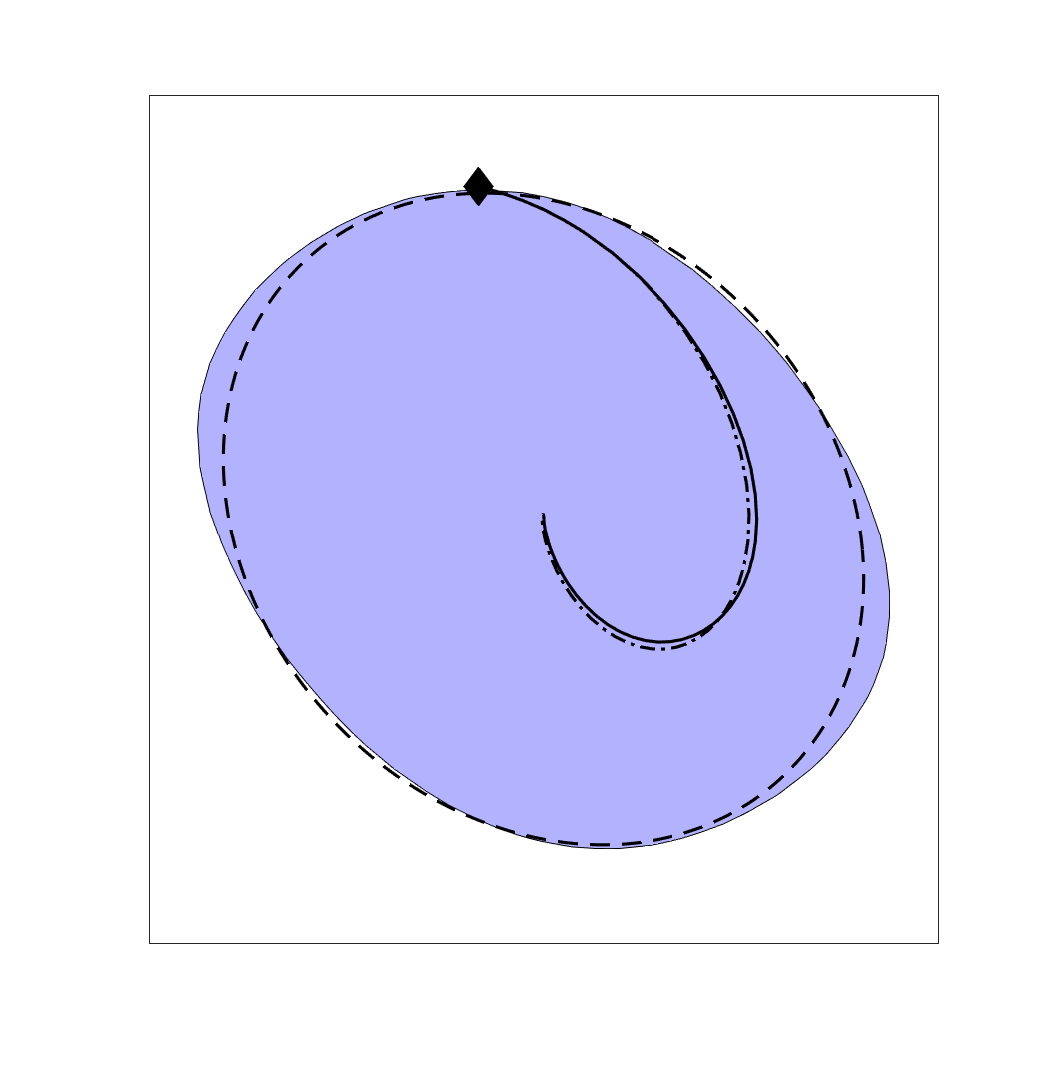
\includegraphics[width=\linewidth]{images/GusevM_pendulum_T=5.eps}};
				\pgfkeys{/pgf/number format/.cd,fixed relative,precision=3}
				\begin{axis}[%
					width=0.772\linewidth,
					height=0.832\linewidth,
					at={(0\linewidth,0\linewidth)},
					scale only axis,
					xmin=-2,
					xmax=2,
					xlabel style={font=\color{white!15!black}},
					ylabel near ticks,
					xlabel={$ x_1 $},
					ymin=-2,
					ymax=2,
					ylabel style={font=\color{white!15!black}},
					ylabel={$ x_2 $},
					xmajorgrids,
					ymajorgrids,
					grid style={dashed, opacity=0.7}
				]
				\end{axis}
			\end{tikzpicture}%
			\subcaption{при $T = 5$;}
			\label{fig:pendulum_T=5} 
		\end{minipage}
		\begin{minipage}[b]{.49\linewidth} 
			\centering
			\begin{tikzpicture}
				\node at (3.16,3.41)
				{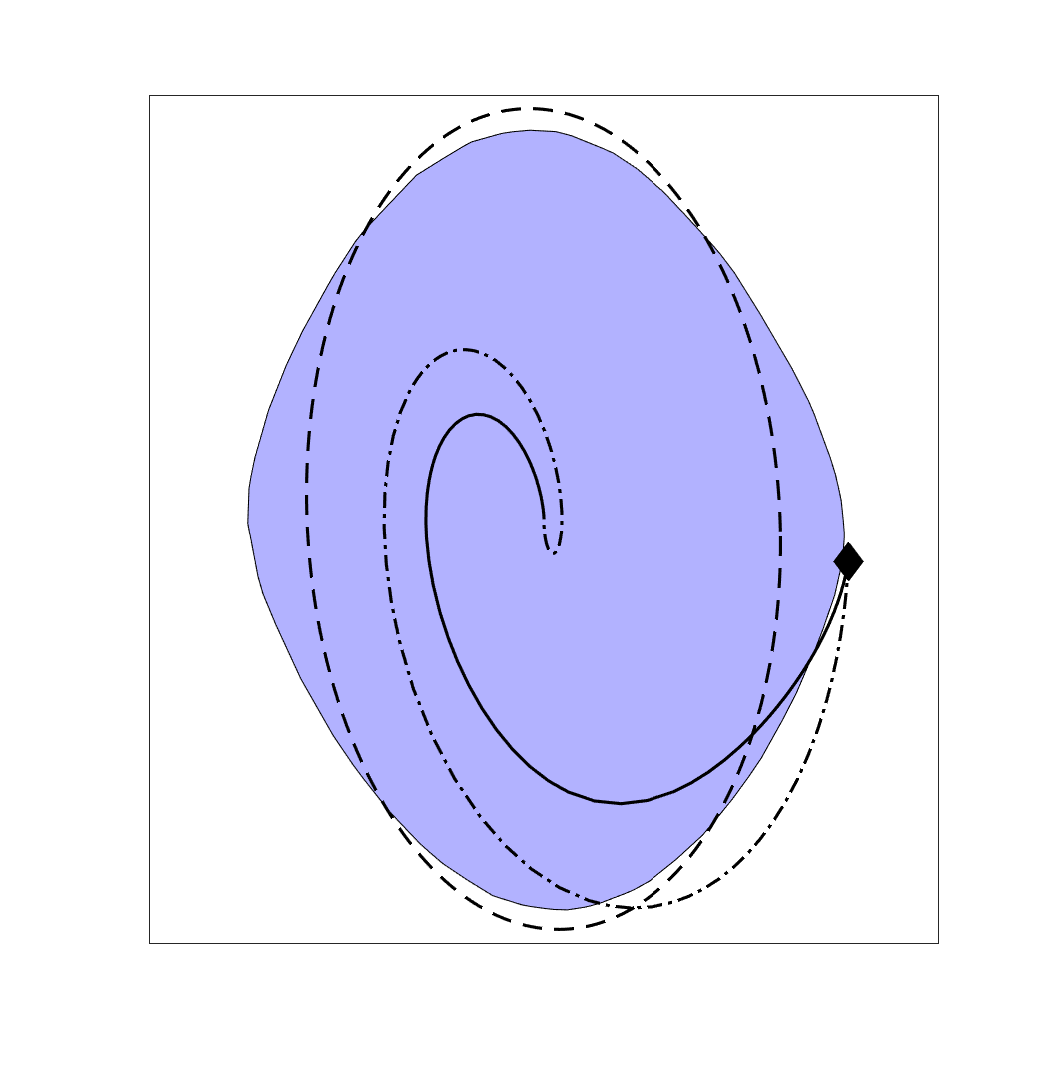
\includegraphics[width=\linewidth]{images/GusevM_pendulum_T=7.eps}};
				\pgfkeys{/pgf/number format/.cd,fixed relative,precision=3}
				\begin{axis}[%
					width=0.772\linewidth,
					height=0.832\linewidth,
					at={(0\linewidth,0\linewidth)},
					scale only axis,
					xmin=-3,
					xmax=3,
					xlabel style={font=\color{white!15!black}},
					ylabel near ticks,
					xlabel={$ x_1 $},
					ymin=-2,
					ymax=2,
					ylabel style={font=\color{white!15!black}},
					ylabel={$ x_2 $},
					xmajorgrids,
					ymajorgrids,
					grid style={dashed, opacity=0.7}
				]
				\end{axis}
			\end{tikzpicture}%
			\subcaption{при $T = 7$;}
			\label{fig:pendulum_T=7}  
		\end{minipage} 
		\caption{Результаты численного эксперимента для систем \eqref{linear_pendulum} и \eqref{pendulum}}\label{fig:pendulum}
	\end{figure}
	 На рисунках  \ref{fig:pendulum}-\subref{fig:pendulum_T=5} и \ref{fig:pendulum}-\subref{fig:pendulum_T=7} приняты следующие обозначения. Пунктирная линия --- граница множества нуль управляемости $N_1(T,1)$ линеаризованной системы \eqref{linear_pendulum}, совпадающего с множеством достижимости $G_1(T,1)$ линейной системы, отвечающей паре $(-A,-B)$. Множество  нуль управляемости $ N_2(T,1) $ нелинейной системы \eqref{pendulum}, которое совпадает с множеством достижимости $G_2(T,1)$ системы $ \dot{x_1} = -x_2, \
		\dot{x_2} = \sin(x_1) - u$ закрашено.   Движение нелинейной системы показано сплошной линией, а линеаризованной --- штрихпунктирной. 
	
	В случае $ T = 5$, множества  $N_1(5,1) $  и $ N_2(5,1) $ систем  близки, как и траектории, приводящие системы из начального состояния $x_0$ (черный ромб) в начало координат.  При $T = 7$, формы множеств $N_1(7,1) $ и  $ N_2(7,1) $ различны, как и траектории систем. Тем не менее, линейная обратная связь приводит нелинейную систему в начало координат.
	Значения начальных состояний $x_0$ и функционалов интегрального ресурса $ \displaystyle{\int_0^T u^{\top}(\tau) u(\tau) \, d\tau}$ в линейном ($ J $) и нелинейном ($ \widetilde{J} $) случае приведены в таблице \ref{Example1_table}.
	\end{pr}
	\begin{table}[h!]
	\begin{center}
	\caption{Результаты численного эксперимента с системами \eqref{linear_pendulum} и \eqref{pendulum}}
	\label{Example1_table}
	\begin{tabular}{c|c|c|c|c|c}
	№       & Время $T$, c    &  $x_0$                  & $ J $                & $ \widetilde{J} $  & $  ( J -  \widetilde{J} ) / J$ \\ \hline
	1       & $0.01 $         & $ (-0.0005; 0.1) $      & $ 1.0000 $           & $ 1.0000 $         &  5.92e-13  \\ \hline %phi = 135 eps = 6e-11
	2       & $ 1 $           & $ (0.1542; -0.6945) $   & $ 1.0000 $           & $ 0.9998 $         &  1.36e-4  \\ \hline %phi = 225 eps = 5e-8
	3       & $ 1 $           & $ (-0.4312; 0.2701) $   & $ 0.9961 $           & $ 0.9997 $         &  $-0.0036$  \\ \hline % phi = 200 eps = 5e-8
	4       & $5 $            & $ (-0.3696; 1.5540) $   & $ 1.0233 $           & $ 0.9983 $         & 0.0244   \\ \hline % eps = 5e-4; phi = 90
	5       & $ 7 $           & $ (2.2886; -0.1012) $   & $ 1.6104 $           & $ 0.9977 $         & 0.3805   %eps = 5e-4; phi = -10
	\end{tabular}
	\end{center}
	\end{table}
	\begin{pr}
	Следующий пример показывает, что описанный выше метод построения обратной связи может быть применен и к системам более общего вида с матрицей при управлении, зависящей от фазовых переменных. В этом случае, условие  асимптотической эквивалентности  множеств достижимости (нуль-управляемости) нелинейной и линеаризованной систем (условие \ref{condC}) следует использовать в виде $ \nu_1(\tau) \geqslant \tau^{1 - \alpha} / k_4^2 $.   Пусть управляемая  система описывается уравнениями
	
	\begin{gather}\label{bilinear}
	\begin{gathered}
		\dot{x_1} = x_2 u_1 - (1 + x_1) u_2, \qquad \dot{x_2} = -(1+x_1) u_1 - x_2 u_2, \\
		0 \leqslant t \leqslant T, \quad
		x(0) = x_0.
		\end{gathered}
	\end{gather}
	
	Желаемое конечное состояние $ x_1(T) = x_2(T) =  0 $. Матрицы линеаризованной в конечной точке системы имеют вид:
	\begin{gather}\label{linear_bilinear}
		A = \begin{pmatrix}
			0 & 0\\
			0 & 0
		\end{pmatrix}, \qquad 
		B = \begin{pmatrix}
			0 & -1 \\
			-1 & 0
		\end{pmatrix}.
	\end{gather}
	 
	Здесь грамиан управляемости $ W_1 $, как и его минимальное собственное число $ \nu_1 $, линейной системы, отвечающий паре  $(-\tau A, -B) $ не зависит от $ \tau $, а значит условие $ \nu_1 \geqslant \tau^{1 - \alpha} / k_4^2 $ выполняется при малых $\tau$. Доказательство, приведенное в предыдущем разделе не распространяется на случай таких систем, но можно показать, что обратная связь \eqref{feedback}, рассчитанная для линейной системы \eqref{linear_bilinear},  также приводит в нуль и систему \eqref{bilinear}. Это и продемонстрировано на рисунках \ref{fig:bilinear}-\subref{fig:bilinear_T=0.1} и \ref{fig:bilinear}-\subref{fig:bilinear_T=3}. Обозначения аналогичны использованным в предыдущем примере. 
	
	При $T = 0.1 $ множества нуль управляемости линейной и нелинейной систем близки. На рисунке \ref{fig:bilinear}-\subref{fig:bilinear_T=0.1} изображены две случая. В обоих начальные состояния выбраны на границе множества нуль управляемости $N_1(0.001,1)$  линеаризованной системы \eqref{linear_bilinear} (множества достижимости $G_1(0.001,1)$ линейной системы, отвечающей паре $(-A,-B)$). В обоих случаях линейная обратная связь приводит в нуль как линейную, так и нелинейную системы. При $ T = 3 $ множества нуль управляемости существенно различаются. Тем не менее, обе системы по-прежнему приводятся в нуль. Значения начальных начальных состояний $x_0$ и функционалов интегрального ресурса $ \displaystyle{\int_0^T u^{\top}(\tau) u(\tau) \, d\tau}$ в линейном ($ J $) и нелинейном ($ \widetilde{J} $) случае  приведены в таблице \ref{Example2_table}.
	\end{pr}
	\begin{table}
	\caption{Результаты численного эксперимента с системами \eqref{linear_bilinear} и   \eqref{bilinear}}
	\label{Example2_table}
	\begin{center}
	\begin{tabular}{c|c|c|c|c|c}
	№       & Время $T$, c    &  $x_0$                  & $ J $                & $ \widetilde{J} $  & $  ( J -  \widetilde{J} ) / J$ \\ \hline
	1       & 1.0e-6          &  (-1.74e-4; 9.85e-4)    & $ 1.0000 $           & $ 1.0001 $         & $-1.73$e-4 \\ \hline %phi = 100 %eps=2е-11
	%2       & $0.001 $        & $ (-0.0311; 0.0055)  $  & $ 1.0000 $           & $ 1.0321 $         & $-0.032$ \\ \hline %phi = 170 %eps=2е-8
	2       & $0.001 $        & $ (0.0311; 0.0055)  $   & $ 1.0000 $           & $ 0.9697 $         & $0.03$ \\ \hline %phi = 10 %eps=2е-8
	%4       & $0.01 $         & $ (0.0985; 0.0174) $    & $ 1.0000 $           & $ 0.9102 $         & $ 0.09$ \\ \hline %phi = 10 %eps=2е-7
	3       & $0.01 $         & $ (-0.0985; -0.0174) $  & $ 1.0000 $           & $ 1.1090 $         &  $-0.11$\\ \hline %phi = 170 %eps=2е-7
	4       & $0.1 $         & $ (-0.2972; 0.1082) $  & $ 1.0000 $           & $ 1.4116 $         &  $-0.4117$\\ \hline %phi = 160 %eps=2е-6
	5       & $0.1 $         & $ (0.2972; 0.1082) $  & $ 1.0000 $           & $ 0.7691  $         &  $0.2308$\\ \hline %phi = 20 %eps=2е-6
	6       & $ 3 $           & $ (-1.2247; 1.2247) $   & $1.0000 $            & $1.4305 $          &  $-0.4305$   \\ \hline %phi = 135 linear %eps=5е-5
	7       & $ 3 $           & $ (1.3813; 3.4640) $    & $4.6356 $            & $1.2960 $          & 0.7204
	%phi = 90 %eps=5е-5
	\end{tabular}
	\end{center}
	\end{table} 
	\begin{figure}[ht!] 
		\begin{minipage}[b]{.49\linewidth} 
			\centering 
			\begin{tikzpicture}
				\node at (3.16,3.41) 
				{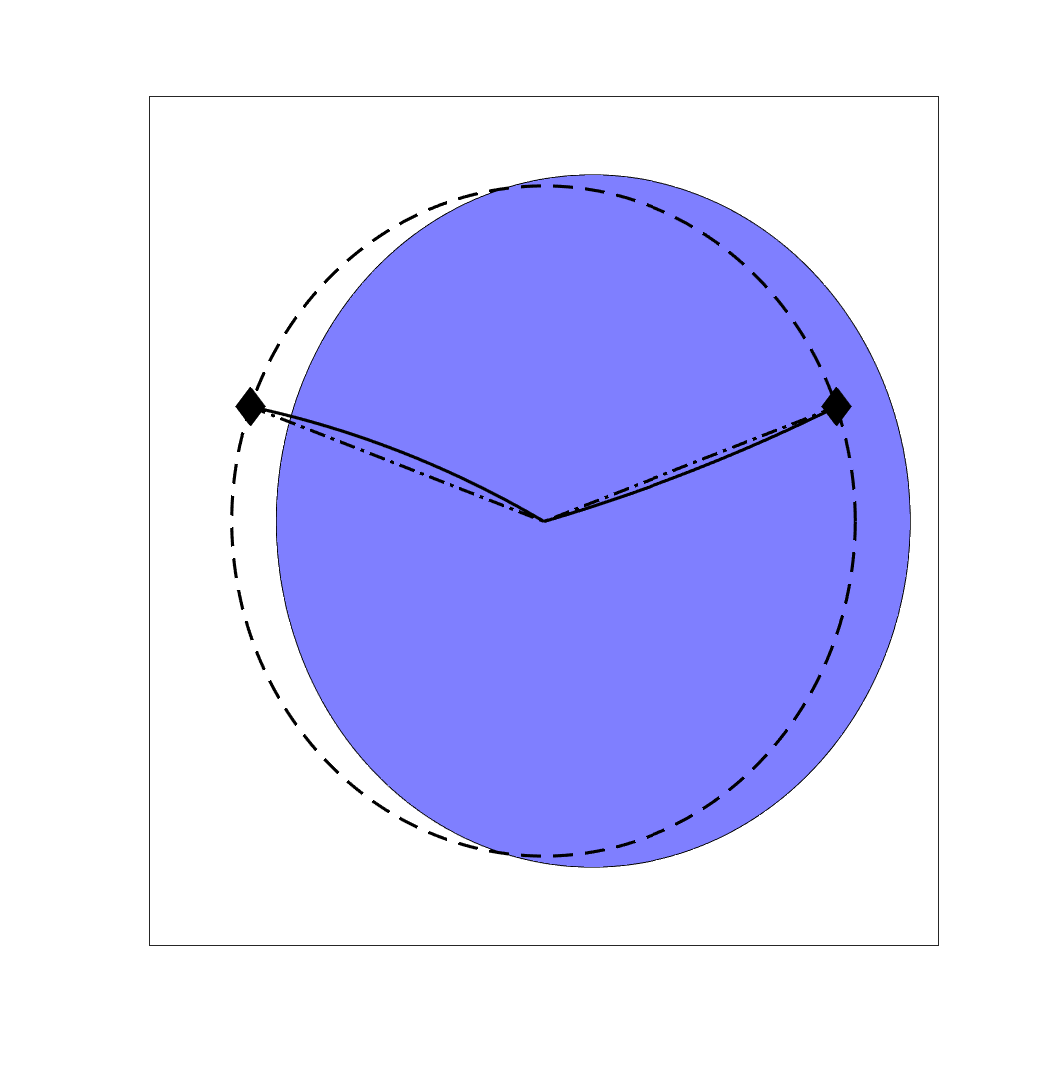
\includegraphics[width=\linewidth]{images/GusevM_bilinear_T=100.eps}};
				\pgfkeys{/pgf/number format/.cd,fixed relative,precision=3}
				\begin{axis}[%
					width=0.772\linewidth,
					height=0.832\linewidth,
					at={(0\linewidth,0\linewidth)},
					scale only axis,
					xmin=-0.4,
					xmax=0.4,
					xlabel style={font=\color{white!15!black}},
					ylabel near ticks,
					xlabel={$ x_1 $},
					ymin=-0.4,
					ymax=0.4,
					ylabel style={font=\color{white!15!black}},
					ylabel={$ x_2 $},
					xmajorgrids,
					ymajorgrids,
					grid style={dashed, opacity=1}
				]
				\end{axis}
			\end{tikzpicture}%
			\subcaption{при $T = 0.1$;}
			\label{fig:bilinear_T=0.1} 
		\end{minipage}
		\begin{minipage}[b]{.49\linewidth} 
			\centering
			\begin{tikzpicture}
				\node at (3.16,3.41) 
				{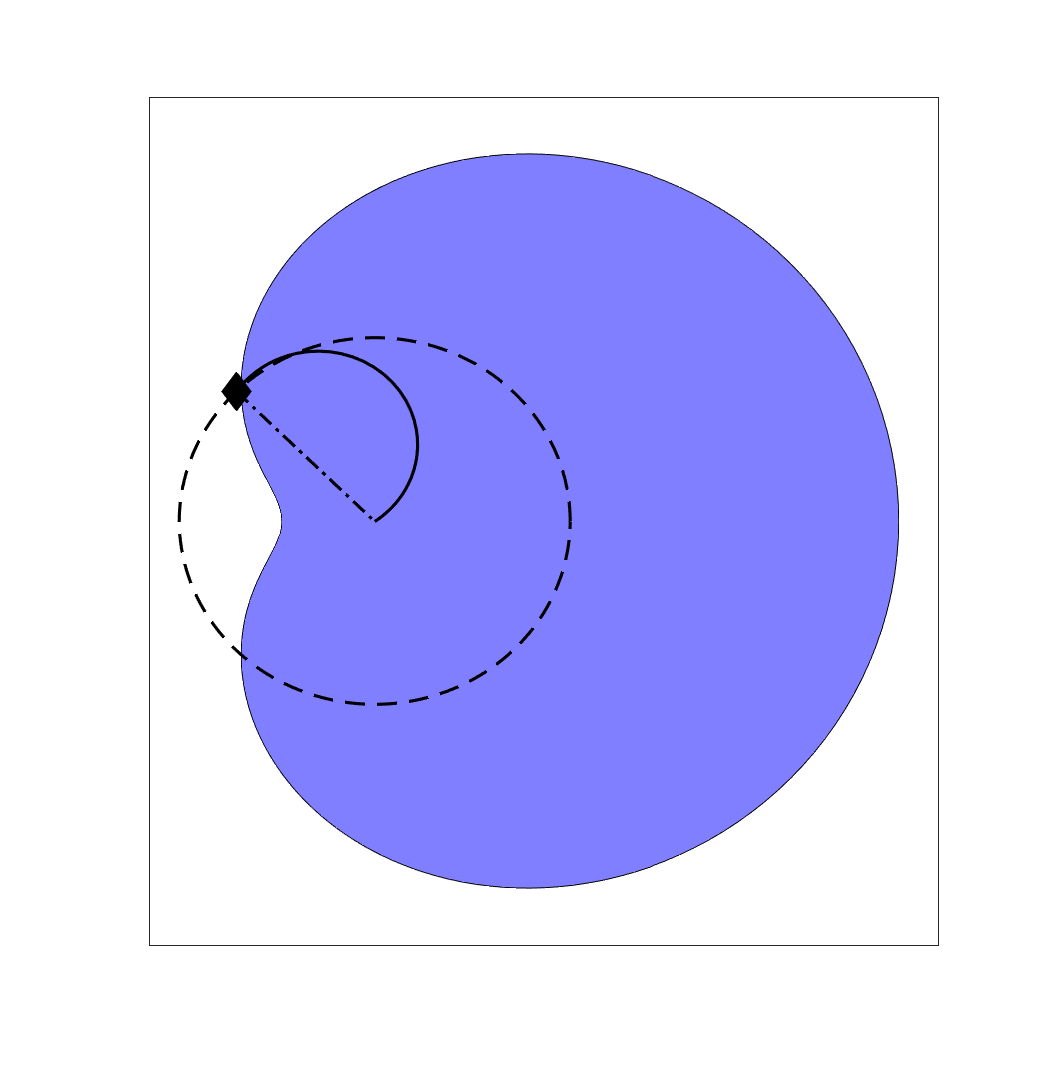
\includegraphics[width=\linewidth]{images/GusevM_bilinear_T=3000.eps}};
				\pgfkeys{/pgf/number format/.cd,fixed relative,precision=3}
				\begin{axis}[%
					width=0.772\linewidth,
					height=0.832\linewidth,
					at={(0\linewidth,0\linewidth)},
					scale only axis,
					xmin=-2,
					xmax=5,
					xlabel style={font=\color{white!15!black}},
					ylabel near ticks,
					xlabel={$ x_1 $},
					ymin=-4,
					ymax=4,
					ylabel style={font=\color{white!15!black}},
					ylabel={$ x_2 $},
					xmajorgrids,
					ymajorgrids,
					grid style={dashed, opacity=1}
				]
				\end{axis}
			\end{tikzpicture}%
			\subcaption{при $T = 3$;}
			\label{fig:bilinear_T=3}  
		\end{minipage} 
		\caption{Результаты численного эксперимента для систем \eqref{linear_bilinear} и   \eqref{bilinear}}\label{fig:bilinear}
	\end{figure}
	
	Можно обратить внимание, что в некоторых экспериментах, описанных в таблицах \ref{Example1_table} и \ref{Example2_table}, значение интегрального функционала в нелинейном случае может быть как меньше, так и больше значения этого же функционала в линейном случае. Это объясняется тем, что нелинейные слагаемые могут как способствовать переводу систему в нуль (тогда значение функционала в нелинейном случае будет меньше), либо препятствовать этому (тогда меньше будет значение линейного функционала в линейном случае). Это явление иллюстрируется следующим примером.
	
	\begin{pr}
	 Рассмотрим две одномерные нелинейные системы
	 \begin{gather*}
		\dot{y} = y + y^3 + u, \quad 
		\dot{z} = z - z^3 + u, \qquad
		0 \leqslant t \leqslant T, \quad
		x(0) = y(0) = z(0) = x_0. 
	\end{gather*}
	Обеим системам в нуле отвечает одна и та же линеаризованная система $ \dot{x} = x + u$. $ Q(t) = 2/(1 - e^{-2(T-t)})$. Обратная связь $ u(x) = -2x/(1 - e^{-2(T-t)})$ приводит в начало координат все три системы. При $T = 1$ и $x_0 = 0.6575$ значение функционала интегрального ресурса в линейном случае равно 1, в случае $y$ --- 1.19, а в случае $z$ --- 0.87. 
	\end{pr}
\end{document}